\apendice{Especificación de Requisitos}

\section{Introducción}
Para comenzar con el desarrollo de la aplicación web sobre la que se basa este proyecto, se debe realizar un estudio de los requisitos que son necesarios cubrir. 
Con estos requisitos se podrán detectar las funcionalidades necesarias y se podrán generar los casos de uso de la aplicación.

Este es el punto de partida para realizar un buen diseño de la aplicación que facilitará las siguientes tareas a realizar.

\section{Objetivos generales}
El objetivo de este proyecto es desarrollar una aplicación web para poder llevar a cabo la gestión de las diferentes áreas de la Universidad de Burgos. El sistema gestionará el profesorado, asignaturas, reconocimiento de docencia...

\section{Catálogo de requisitos}
A continuación se van a exponer los requisitos de la aplicación web.
\subsection{Requisitos funcionales}
\begin{enumerate}
	\item \textbf{RF-01.} Mantenimiento de titulaciones.\label{itm:RF1}
	\item \textbf{RF-02.} Mantenimiento de asignaturas.\label{itm:RF2}
	\item \textbf{RF-03.} Mantenimiento de grupos.\label{itm:RF3}
	\item \textbf{RF-04.} Mantenimiento de docentes.\label{itm:RF4}
	\item \textbf{RF-05.} Mantenimiento de centros.\label{itm:RF5}
	\item \textbf{RF-06.} Mantenimiento de cursos académicos.\label{itm:RF6}
	\item \textbf{RF-07.} Mantenimiento de plazas.\label{itm:RF7}
	\item \textbf{RF-08.} Mantenimiento de tipos de contrato.\label{itm:RF8}
	\item \textbf{RF-09.} Mantenimiento de áreas.\label{itm:RF9}
	\item \textbf{RF-10.} Mantenimiento de departamentos.\label{itm:RF10}
	\item \textbf{RF-11.} Un administrativo puede asignar horas a un docente (plaza) en un grupo de un curso.\label{itm:RF11}
	\item \textbf{RF-12.} Un administrativo puede asignar una plaza a un docente.\label{itm:RF12}
	\item \textbf{RF-13.} Un grupo puede ser asignado a una asignatura en un curso.\label{itm:RF13}
\end{enumerate}

\subsection{Requisitos no funcionales}
\begin{itemize}
	\item \textbf{RNF-01.} El sistema debe ser fácil de usar.
	\item \textbf{RNF-02.} El sistema no debe permitir el acceso no autorizado.

\end{itemize}

\clearpage
\section{Especificación de requisitos}
\subsection{Casos de uso}
\begin{figure}[!h]
	\centering
	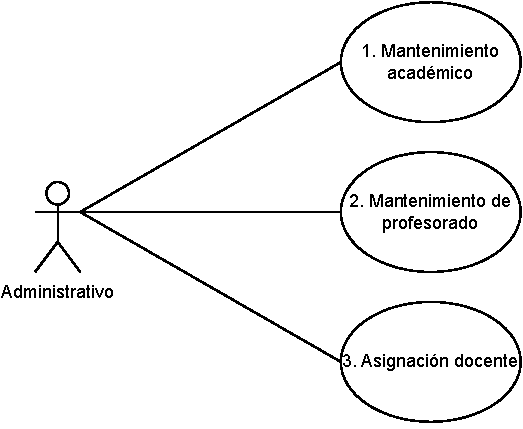
\includegraphics[scale=0.85]{../img/Anexos/Casos uso/Diagrama casos de uso 1.pdf}
	\caption{Diagrama de casos de uso general}
\end{figure}
\FloatBarrier

\subsubsection{1. Mantenimiento académico}
\begin{figure}[!h]
	\centering
	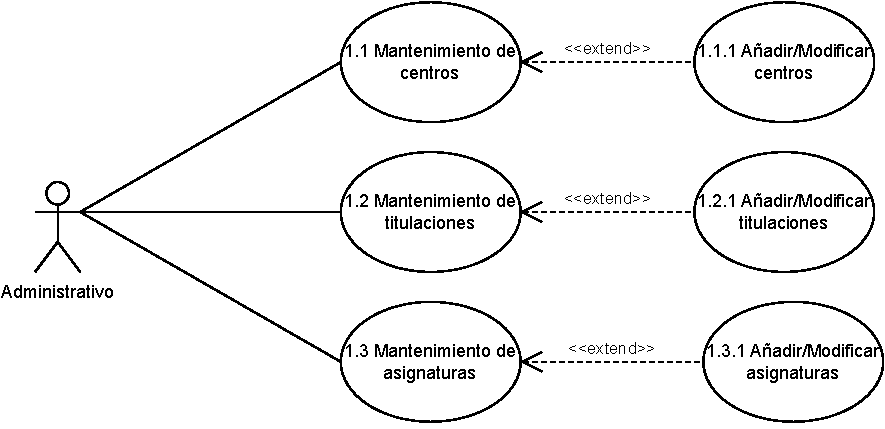
\includegraphics[scale=0.85]{../img/Anexos/Casos uso/Diagrama casos de uso 2.pdf}
	\caption{Diagrama de caso de uso - 1. Mantenimiento académico}
\end{figure}
\FloatBarrier

\begin{table}[p]
\label{table:CU-1}
	\centering
	\begin{tabularx}{\linewidth}{ p{0.21\columnwidth} p{0.71\columnwidth} }
		\toprule
		\textbf{CU-1}    & \textbf{Mantenimiento académico}\\
		\toprule
		\textbf{Versión}              & 1.0    \\
		\textbf{Autor}                & Ignacio Dávila García \\
		\textbf{Requisitos asociados} & \hyperref[itm:RF5]{RF-05}, \hyperref[itm:RF1]{RF-01}, \hyperref[itm:RF2]{RF-02} \\
		\textbf{Descripción}          & Un administrativo puede realizar labores de mantenimiento de los centros, titulaciones y asignaturas \\
		\textbf{Precondición}         & Tener iniciada sesión con una cuenta con permisos administrativos \\
		\textbf{Acciones}             &
		\begin{enumerate}
			\def\labelenumi{\arabic{enumi}.}
			\tightlist
			\item Seleccionar la opción <<Asignaturas>> del menú principal de la web.
			\item Se abre la ventana de mantenimiento de las asignaturas.
		\end{enumerate}\\
		\textbf{Postcondición}        & Ninguna \\
		\textbf{Excepciones}          & También es posible acceder la ventana de mantenimiento de centros y titulaciones seleccionando las opciones <<Centros>> (\hyperref[table:CU-1.1]{CU-1.1}) o <<Titulaciones>> (\hyperref[table:CU-1.2]{CU-1.2}) respectivamente. Si no se pulsa ninguna, se permanece en la ventana actual. \\
		\textbf{Importancia}          & Alta \\
		\bottomrule
	\end{tabularx}
	\caption{CU-1 Mantenimiento académico.}
\end{table}
\FloatBarrier

\begin{table}[p]
\label{table:CU-1.1}
	\centering
	\begin{tabularx}{\linewidth}{ p{0.21\columnwidth} p{0.71\columnwidth} }
		\toprule
		\textbf{CU-1.1}    & \textbf{Mantenimiento de centros}\\
		\toprule
		\textbf{Versión}              & 1.0    \\
		\textbf{Autor}                & Ignacio Dávila García \\
		\textbf{Requisitos asociados} & \hyperref[itm:RF5]{RF-05} \\
		\textbf{Descripción}          & Un administrativo puede realizar el mantenimiento de los centros \\
		\textbf{Precondición}         & Realizar el~\hyperref[table:CU-1]{CU-1} \\
		\textbf{Acciones}             &
		\begin{enumerate}
			\def\labelenumi{\arabic{enumi}.}
			\tightlist
			\item Se abre una ventana donde aparece una tabla con los centros creados desde donde se podrá realizar el mantenimiento.
		\end{enumerate}\\
		\textbf{Postcondición}        & Ninguna \\
		\textbf{Excepciones}          & Si se pulsa sobre el botón <<Nuevo>>, se accede a la creación de centros (\hyperref[table:CU-1.1.1]{CU-1.1.1}). Si se pulsa sobre el botón <<Modificar>> de un centro del listado, se accede a la ventana de modificación del centro. Por último, si se pulsa sobre el botón <<Eliminar>> de un centro el sistema pregunta si está seguro, y al pulsar en <<Sí>>, este se elimina produciendo un borrado en cascada de las titulaciones vinculadas. \\
		\textbf{Importancia}          & Alta \\
		\bottomrule
	\end{tabularx}
	\caption{CU-1.1 Mantenimiento de centros.}
\end{table}
\FloatBarrier

\begin{table}[p]
\label{table:CU-1.1.1}
	\centering
	\begin{tabularx}{\linewidth}{ p{0.21\columnwidth} p{0.71\columnwidth} }
		\toprule
		\textbf{CU-1.1.1}    & \textbf{Añadir/Modificar centros}\\
		\toprule
		\textbf{Versión}              & 1.0    \\
		\textbf{Autor}                & Ignacio Dávila García \\
		\textbf{Requisitos asociados} & \hyperref[itm:RF5]{RF-05} \\
		\textbf{Descripción}          & Un administrativo añade o modifica un nuevo centro \\
		\textbf{Precondición}         & Realizar el~\hyperref[table:CU-1.1]{CU-1.1} \\
		\textbf{Acciones}             &
		\begin{enumerate}
			\def\labelenumi{\arabic{enumi}.}
			\tightlist
			\item Se abre una ventana con un formulario vacío donde aparecen los campos de la tabla <<Centro>> de la figura \ref{er_cu1}, necesarios para crear un centro.
			\item Rellenar el formulario con los datos del centro que se desea añadir.
			\item Pulsar sobre el botón <<Añadir>>.
		\end{enumerate}\\
		\textbf{Postcondición}        & El centro queda añadido/modificado y el sistema lleva al usuario a la ventana de centros donde se puede ver el listado de todos los centros creados. \\
		\textbf{Excepciones}          & Se dejan campos vacíos o se introducen datos con un formato incorrecto. Otra forma de finalizar el caso de uso es la modificación. En este caso, se pulsa sobre el botón <<Modificar>> de un centro y se accede al mismo formulario con los campos rellenos. Finalmente se pulsa en el botón <<Modificar>> \\
		\textbf{Importancia}          & Alta \\
		\bottomrule
	\end{tabularx}
	\caption{CU-1.1.1 Añadir/Modificar centros.}
\end{table}
\FloatBarrier

\begin{table}[p]
\label{table:CU-1.2}
	\centering
	\begin{tabularx}{\linewidth}{ p{0.21\columnwidth} p{0.71\columnwidth} }
		\toprule
		\textbf{CU-1.2}    & \textbf{Mantenimiento de titulaciones}\\
		\toprule
		\textbf{Versión}              & 1.0    \\
		\textbf{Autor}                & Ignacio Dávila García \\
		\textbf{Requisitos asociados} & \hyperref[itm:RF1]{RF-01} \\
		\textbf{Descripción}          & Un administrativo puede realizar el mantenimiento de las titulaciones \\
		\textbf{Precondición}         & Realizar el~\hyperref[table:CU-1]{CU-1} \\
		\textbf{Acciones}             &
		\begin{enumerate}
			\def\labelenumi{\arabic{enumi}.}
			\tightlist
			\item Se abre una ventana donde aparece una tabla con las titulaciones creadas desde donde se podrá realizar el mantenimiento.
		\end{enumerate}\\
		\textbf{Postcondición}        & Ninguna \\
		\textbf{Excepciones}          & Si se pulsa sobre el botón <<Nuevo>>, se accede a la creación de titulaciones (\hyperref[table:CU-1.2.1]{CU-1.2.1}). Si se pulsa sobre el botón <<Modificar>> de una titulación de la lista se accede a la ventana de modificación. Por último, si se pulsa sobre el botón <<Eliminar>> de una titulación el sistema pregunta si está seguro, y al pulsar en <<Sí>>, esta se elimina produciendo un borrado en cascada de las asignaturas vinculadas. \\
		\textbf{Importancia}          & Alta \\
		\bottomrule
	\end{tabularx}
	\caption{CU-1.2 Mantenimiento de titulaciones.}
\end{table}
\FloatBarrier

\begin{table}[p]
\label{table:CU-1.2.1}
	\centering
	\begin{tabularx}{\linewidth}{ p{0.21\columnwidth} p{0.71\columnwidth} }
		\toprule
		\textbf{CU-1.2.1}    & \textbf{Añadir/Modificar titulaciones}\\
		\toprule
		\textbf{Versión}              & 1.0    \\
		\textbf{Autor}                & Ignacio Dávila García \\
		\textbf{Requisitos asociados} & \hyperref[itm:RF1]{RF-01} \\
		\textbf{Descripción}          & Un administrativo añade o modifica una titulación \\
		\textbf{Precondición}         & Realizar el~\hyperref[table:CU-1.2]{CU-1.2} y tener algún centro creado \\
		\textbf{Acciones}             &
		\begin{enumerate}
			\def\labelenumi{\arabic{enumi}.}
			\tightlist
			\item Se abre una ventana con un formulario vacío donde aparecen los campos de la tabla <<Titulación>> de la figura \ref{er_cu1}, necesarios para crear una titulación. También aparece el campo <<Centro>> para seleccionar el centro al que pertenece.
			\item Rellenar el formulario con los datos de la titulación que se desea añadir.
			\item Pulsar sobre el botón <<Añadir>>.
		\end{enumerate}\\
		\textbf{Postcondición}        & La titulación queda añadida/modificada y el sistema lleva al usuario a la ventana de titulaciones donde se puede ver el listado de todos las titulaciones añadidas. \\
		\textbf{Excepciones}          & Se dejan campos vacíos o se introducen datos con un formato incorrecto. Otra forma de finalizar el caso de uso es la modificación. En este caso, se pulsa sobre el botón <<Modificar>> de una titulación de la tabla y se accede al mismo formulario, pero con los campos rellenos. Finalmente se pulsa en el botón <<Modificar>> y la titulación queda modificada. \\
		\textbf{Importancia}          & Alta \\
		\bottomrule
	\end{tabularx}
	\caption{CU-1.2.1 Añadir/Modificar centros.}
\end{table}
\FloatBarrier

\begin{table}[p]
\label{table:CU-1.3}
	\centering
	\begin{tabularx}{\linewidth}{ p{0.21\columnwidth} p{0.71\columnwidth} }
		\toprule
		\textbf{CU-1.3}    & \textbf{Mantenimiento de asignaturas}\\
		\toprule
		\textbf{Versión}              & 1.0    \\
		\textbf{Autor}                & Ignacio Dávila García \\
		\textbf{Requisitos asociados} & \hyperref[itm:RF2]{RF-02} \\
		\textbf{Descripción}          & Un administrativo puede realizar el mantenimiento de asignaturas \\
		\textbf{Precondición}         & Realizar el~\hyperref[table:CU-1]{CU-1} \\
		\textbf{Acciones}             &
		\begin{enumerate}
			\def\labelenumi{\arabic{enumi}.}
			\tightlist
			\item Se abre una ventana donde aparece una tabla con las asignaturas creadas desde donde se podrá realizar el mantenimiento.
		\end{enumerate}\\
		\textbf{Postcondición}        & Ninguna \\
		\textbf{Excepciones}          & Si se pulsa sobre el botón <<Nuevo>>, se accede a la creación de asignaturas (\hyperref[table:CU-1.3.1]{CU-1.3.1}). Si se pulsa sobre el botón <<Modificar>> de una asignaturas de la lista se accede a la ventana de modificación. Por último, si se pulsa sobre el botón <<Eliminar>> de una asignatura el sistema pregunta si está seguro, y al pulsar en <<Sí>> esta se elimina. \\
		\textbf{Importancia}          & Alta \\
		\bottomrule
	\end{tabularx}
	\caption{CU-1.3 Mantenimiento de asignaturas.}
\end{table}
\FloatBarrier

\begin{table}[p]
\label{table:CU-1.3.1}
	\centering
	\begin{tabularx}{\linewidth}{ p{0.21\columnwidth} p{0.71\columnwidth} }
		\toprule
		\textbf{CU-1.3.1}    & \textbf{Añadir/Modificar asignaturas}\\
		\toprule
		\textbf{Versión}              & 1.0    \\
		\textbf{Autor}                & Ignacio Dávila García \\
		\textbf{Requisitos asociados} & \hyperref[itm:RF2]{RF-02} \\
		\textbf{Descripción}          & Un administrativo añade o modifica una asignatura \\
		\textbf{Precondición}         & Realizar el~\hyperref[table:CU-1.3]{CU-1.3} y tener alguna titulación creada \\
		\textbf{Acciones}             &
		\begin{enumerate}
			\def\labelenumi{\arabic{enumi}.}
			\tightlist
			\item Se abre una ventana con un formulario vacío donde aparecen los campos de la tabla <<Asignatura>> de la figura \ref{er_cu1}, necesarios para crear una asignatura. También se debe indicar la titulación a la que pertenece y rellenar el campo <<Abreviatura>> que permite la selección múltiple de abreviaturas separadas por comas. Las abreviaturas existentes aparecen al escribir y se pueden seleccionar. Si se escribe una nueva se almacena.
			\item Rellenar el formulario con los datos de la asignatura que se desea añadir.
			\item Pulsar sobre el botón <<Añadir>>.
		\end{enumerate}\\
		\textbf{Postcondición}        & La asignatura queda añadida/modificada y el sistema lleva al usuario a la ventana de asignaturas donde se puede ver el listado de todos las asignaturas añadidas. \\
		\textbf{Excepciones}          & Se dejan campos vacíos, se introducen datos con un formato incorrecto o se introduce una id existente. Otra forma de finalizar el caso de uso es la modificación. En este caso, se pulsa sobre el botón <<Modificar>> de una asignatura de la tabla y se accede al mismo formulario, pero con los campos rellenos. Finalmente se pulsa en el botón <<Modificar>> y la asignatura queda modificada. \\
		\textbf{Importancia}          & Alta \\
		\bottomrule
	\end{tabularx}
	\caption{CU-1.3.1 Añadir/Modificar asignaturas.}
\end{table}
\FloatBarrier

\begin{figure}[!h]
	\centering
	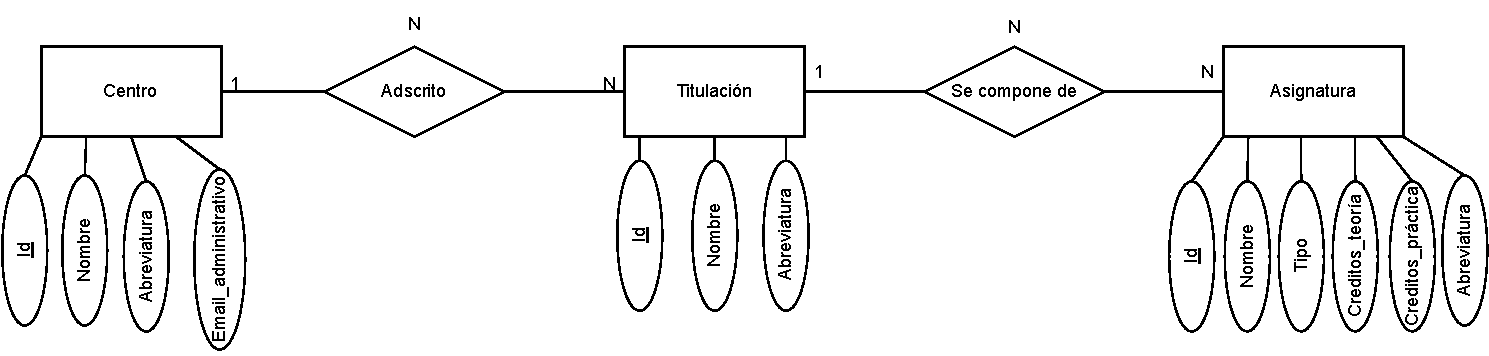
\includegraphics[scale=0.75]{../img/Anexos/Casos uso/Vistas ER/Diagrama E-R CU 1.pdf}
	\caption{Vista diagrama entidad relación para el CU-1}
	\label{er_cu1}
\end{figure}
\FloatBarrier

\newpage
\subsubsection{2. Mantenimiento de profesorado}
\begin{figure}[!h]
	\centering
	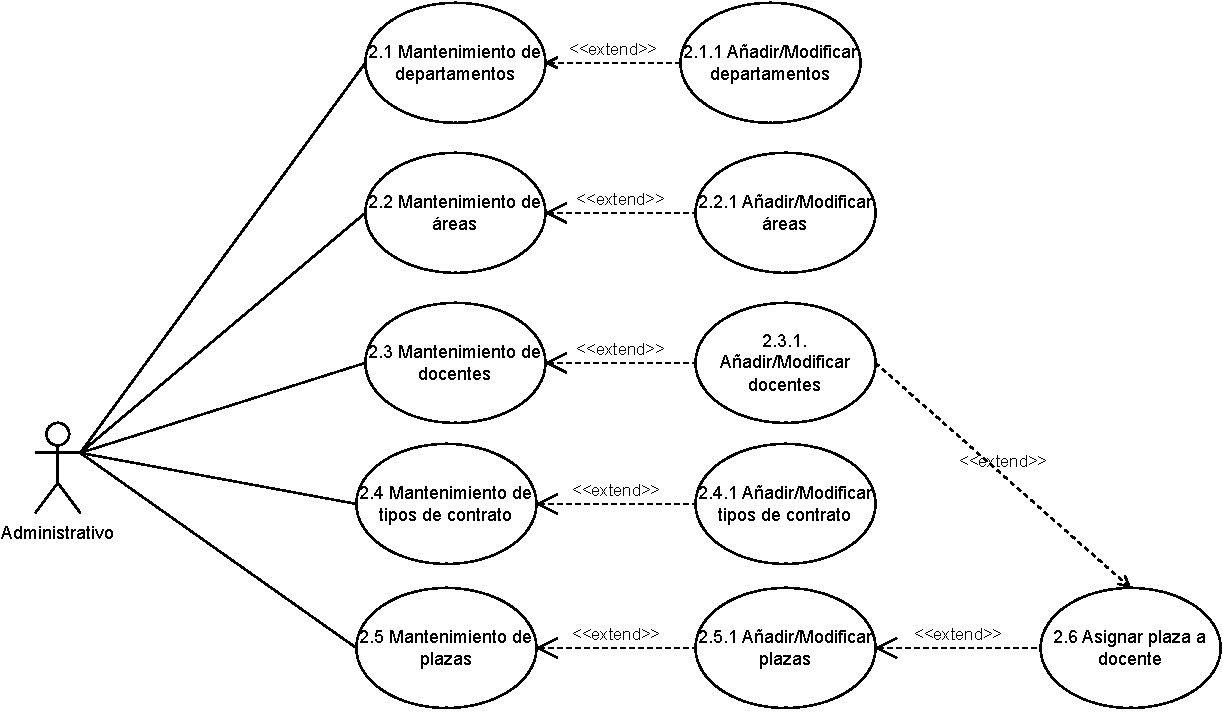
\includegraphics[scale=0.75]{../img/Anexos/Casos uso/Diagrama casos de uso 3.pdf}
	\caption{Diagrama de caso de uso - 2. Mantenimiento de profesorado}
\end{figure}
\FloatBarrier

\begin{table}[p]
\label{table:CU-2}
	\centering
	\begin{tabularx}{\linewidth}{ p{0.21\columnwidth} p{0.71\columnwidth} }
		\toprule
		\textbf{CU-2}    & \textbf{Mantenimiento de profesorado}\\
		\toprule
		\textbf{Versión}              & 1.0    \\
		\textbf{Autor}                & Ignacio Dávila García \\
		\textbf{Requisitos asociados} & \hyperref[itm:RF4]{RF-04}, \hyperref[itm:RF7]{RF-07}, \hyperref[itm:RF8]{RF-08}, \hyperref[itm:RF9]{RF-09}, \hyperref[itm:RF10]{RF-10} \\
		\textbf{Descripción}          & Un administrativo puede realizar labores de mantenimiento de los docentes, tipos de contrato, departamentos, áreas y plazas. Además, un administrativo puede asignar una plaza a un docente. \\
		\textbf{Precondición}         & Tener iniciada sesión con una cuenta con permisos administrativos \\
		\textbf{Acciones}             &
		\begin{enumerate}
			\def\labelenumi{\arabic{enumi}.}
			\tightlist
			\item Seleccionar la opción <<Plazas>> del menú principal de la web.
			\item Se abre la ventana de mantenimiento de plazas.
		\end{enumerate}\\
		\textbf{Postcondición}        & El sistema lleva al usuario a la ventana de la opción pulsada. \\
		\textbf{Excepciones}          & Otras opciones que se pueden seleccionar son <<Docentes>> (\hyperref[table:CU-2.3]{CU-2.3}), <<Contratos>> (\hyperref[table:CU-2.4]{CU-2.4}), <<Departamentos>> (\hyperref[table:CU-2.1]{CU-2.1}) o <<Áreas>> (\hyperref[table:CU-2.2]{CU-2.2}). Al seleccionar alguna de estas opciones el sistema lleva al usuario a la ventana de mantenimiento de la opción elegida.  \\
		\textbf{Importancia}          & Alta \\
		\bottomrule
	\end{tabularx}
	\caption{CU-2 Mantenimiento de profesorado.}
\end{table}
\FloatBarrier

\begin{table}[p]
\label{table:CU-2.1}
	\centering
	\begin{tabularx}{\linewidth}{ p{0.21\columnwidth} p{0.71\columnwidth} }
		\toprule
		\textbf{CU-2.1}    & \textbf{Mantenimiento de departamentos}\\
		\toprule
		\textbf{Versión}              & 1.0    \\
		\textbf{Autor}                & Ignacio Dávila García \\
		\textbf{Requisitos asociados} & \hyperref[itm:RF10]{RF-10} \\
		\textbf{Descripción}          & Un administrativo puede realizar el mantenimiento de departamentos \\
		\textbf{Precondición}         & Realizar el~\hyperref[table:CU-2]{CU-2} \\
		\textbf{Acciones}             &
		\begin{enumerate}
			\def\labelenumi{\arabic{enumi}.}
			\tightlist
			\item Se abre una ventana donde aparece una tabla con los departamentos creados desde donde se podrá realizar el mantenimiento.
		\end{enumerate}\\
		\textbf{Postcondición}        & Ninguna \\
		\textbf{Excepciones}          & Si se pulsa sobre el botón <<Nuevo>>, se accede a la creación de departamentos (\hyperref[table:CU-2.1.1]{CU-2.1.1}). Si se pulsa sobre el botón <<Modificar>> de un departamento de la lista, se accede a la ventana de modificación. Por último, si se pulsa sobre el botón <<Eliminar>> de un departamento el sistema pregunta si está seguro, y al pulsar en <<Sí>>, este se elimina produciendo un borrado en cascada de las áreas asociadas. \\
		\textbf{Importancia}          & Alta \\
		\bottomrule
	\end{tabularx}
	\caption{CU-2.1 Mantenimiento de departamentos.}
\end{table}
\FloatBarrier

\begin{table}[p]
\label{table:CU-2.1.1}
	\centering
	\begin{tabularx}{\linewidth}{ p{0.21\columnwidth} p{0.71\columnwidth} }
		\toprule
		\textbf{CU-2.1.1}    & \textbf{Añadir/Modificar departamentos}\\
		\toprule
		\textbf{Versión}              & 1.0    \\
		\textbf{Autor}                & Ignacio Dávila García \\
		\textbf{Requisitos asociados} & \hyperref[itm:RF10]{RF-10} \\
		\textbf{Descripción}          & Un administrativo añade o modifica un departamento \\
		\textbf{Precondición}         & Realizar el~\hyperref[table:CU-2.1]{CU-2.1} \\
		\textbf{Acciones}             &
		\begin{enumerate}
			\def\labelenumi{\arabic{enumi}.}
			\tightlist
			\item Se abre una ventana con un formulario vacío donde aparecen los campos de la tabla <<Departamento>> de la figura \ref{er_cu2}, necesarios para crear un departamento.
			\item Rellenar el formulario con los datos del departamento que se desea añadir.
			\item Pulsar sobre el botón <<Añadir>>.
		\end{enumerate}\\
		\textbf{Postcondición}        & El departamento queda añadido/modificado y el sistema lleva al usuario a la ventana de departamentos donde se puede ver el listado de todos los departamento añadidos. \\
		\textbf{Excepciones}          & Se dejan campos vacíos o se introducen datos con un formato incorrecto. Otra forma de finalizar el caso de uso es la modificación. En este caso, se pulsa sobre el botón <<Modificar>> de un departamento de la tabla y se accede al mismo formulario, pero con los campos rellenos. Finalmente se pulsa en el botón <<Modificar>> y el departamento queda modificado. \\
		\textbf{Importancia}          & Alta \\
		\bottomrule
	\end{tabularx}
	\caption{CU-2.1.1 Añadir/Modificar departamentos.}
\end{table}
\FloatBarrier

\begin{table}[p]
\label{table:CU-2.2}
	\centering
	\begin{tabularx}{\linewidth}{ p{0.21\columnwidth} p{0.71\columnwidth} }
		\toprule
		\textbf{CU-2.2}    & \textbf{Mantenimiento de áreas}\\
		\toprule
		\textbf{Versión}              & 1.0    \\
		\textbf{Autor}                & Ignacio Dávila García \\
		\textbf{Requisitos asociados} & \hyperref[itm:RF9]{RF-09} \\
		\textbf{Descripción}          & Un administrativo puede realizar el mantenimiento de áreas \\
		\textbf{Precondición}         & Realizar el~\hyperref[table:CU-2]{CU-2} \\
		\textbf{Acciones}             &
		\begin{enumerate}
			\def\labelenumi{\arabic{enumi}.}
			\tightlist
			\item Se abre una ventana donde aparece una tabla con las áreas creadas desde donde se podrá realizar el mantenimiento.
		\end{enumerate}\\
		\textbf{Postcondición}        & Ninguna \\
		\textbf{Excepciones}          & Si se pulsa sobre el botón <<Nuevo>>, se accede a la creación de áreas (\hyperref[table:CU-2.2.1]{CU-2.2.1}). Si se pulsa sobre el botón <<Modificar>> de un área de la lista, se accede a la ventana de modificación. Por último, si se pulsa sobre el botón <<Eliminar>> de un área el sistema pregunta si está seguro, y al pulsar en <<Sí>>, esta se elimina produciendo un borrado en cascada de las plazas asociadas. \\
		\textbf{Importancia}          & Alta \\
		\bottomrule
	\end{tabularx}
	\caption{CU-2.2 Mantenimiento de áreas.}
\end{table}
\FloatBarrier

\begin{table}[p]
\label{table:CU-2.2.1}
	\centering
	\begin{tabularx}{\linewidth}{ p{0.21\columnwidth} p{0.71\columnwidth} }
		\toprule
		\textbf{CU-2.2.1}    & \textbf{Añadir/Modificar áreas}\\
		\toprule
		\textbf{Versión}              & 1.0    \\
		\textbf{Autor}                & Ignacio Dávila García \\
		\textbf{Requisitos asociados} & \hyperref[itm:RF9]{RF-09} \\
		\textbf{Descripción}          & Un administrativo añade o modifica un área \\
		\textbf{Precondición}         & Realizar el~\hyperref[table:CU-2]{CU-2} y tener algún departamento creado \\
		\textbf{Acciones}             &
		\begin{enumerate}
			\def\labelenumi{\arabic{enumi}.}
			\tightlist
			\item Se abre una ventana con un formulario vacío donde aparecen los campos de la tabla <<Área>> de la figura \ref{er_cu2}, necesarios para crear un área. También se debe indicar el departamento al que pertenece el área.
			\item Rellenar el formulario con los datos del área que se desea añadir.
			\item Pulsar sobre el botón <<Añadir>>.
		\end{enumerate}\\
		\textbf{Postcondición}        & El área queda añadido/modificado y el sistema lleva al usuario a la ventana de áreas donde se puede ver el listado de todas las áreas añadidas. \\
		\textbf{Excepciones}          & Se dejan campos vacíos o se introducen datos con un formato incorrecto. Otra forma de finalizar el caso de uso es la modificación. En este caso, se pulsa sobre el botón <<Modificar>> de un área de la tabla y se accede al mismo formulario, pero con los campos rellenos. Finalmente se pulsa en el botón <<Modificar>> y el área queda modificada. \\
		\textbf{Importancia}          & Alta \\
		\bottomrule
	\end{tabularx}
	\caption{CU-2.2.1 Añadir/Modificar áreas.}
\end{table}
\FloatBarrier

\begin{table}[p]
\label{table:CU-2.3}
	\centering
	\begin{tabularx}{\linewidth}{ p{0.21\columnwidth} p{0.71\columnwidth} }
		\toprule
		\textbf{CU-2.3}    & \textbf{Mantenimiento de docentes}\\
		\toprule
		\textbf{Versión}              & 1.0    \\
		\textbf{Autor}                & Ignacio Dávila García \\
		\textbf{Requisitos asociados} & \hyperref[itm:RF4]{RF-04} \\
		\textbf{Descripción}          & Un administrativo puede realizar el mantenimiento de docentes \\
		\textbf{Precondición}         & Realizar el~\hyperref[table:CU-2]{CU-2} \\
		\textbf{Acciones}             &
		\begin{enumerate}
			\def\labelenumi{\arabic{enumi}.}
			\tightlist
			\item Seleccionar la opción <<Docentes>> del menú principal de la web.
			\item Se abre una ventana donde aparece una tabla con los docentes creados desde donde se podrá realizar el mantenimiento.
		\end{enumerate}\\
		\textbf{Postcondición}        & Ninguna \\
		\textbf{Excepciones}          & Si se pulsa sobre el botón <<Nuevo>>, se accede a la creación de docentes (\hyperref[table:CU-2.3.1]{CU-2.3.1}). Si se pulsa sobre el botón <<Modificar>> de un docente de la lista, se accede a la ventana de modificación. Por último, si se pulsa sobre el botón <<Eliminar>> de un docente el sistema pregunta si está seguro, y al pulsar en <<Sí>>, este se elimina. \\
		\textbf{Importancia}          & Alta \\
		\bottomrule
	\end{tabularx}
	\caption{CU-2.3 Mantenimiento de docentes.}
\end{table}
\FloatBarrier

\begin{table}[p]
\label{table:CU-2.3.1}
	\centering
	\begin{tabularx}{\linewidth}{ p{0.21\columnwidth} p{0.71\columnwidth} }
		\toprule
		\textbf{CU-2.3.1}    & \textbf{Añadir/Modificar docentes}\\
		\toprule
		\textbf{Versión}              & 1.0    \\
		\textbf{Autor}                & Ignacio Dávila García \\
		\textbf{Requisitos asociados} & \hyperref[itm:RF4]{RF-04} \\
		\textbf{Descripción}          & Un administrativo añade o modifica un docente \\
		\textbf{Precondición}         & Realizar el~\hyperref[table:CU-2.3]{CU-2.3} \\
		\textbf{Acciones}             &
		\begin{enumerate}
			\def\labelenumi{\arabic{enumi}.}
			\tightlist
			\item Se abre una ventana con un formulario vacío donde aparecen los campos de la tabla <<Docente>> de la figura \ref{er_cu2}, necesarios para crear un docente.
			\item Rellenar el formulario con los datos del docente que se desea añadir.
			\item Pulsar sobre el botón <<Añadir>>.
		\end{enumerate}\\
		\textbf{Postcondición}        & El docente queda añadido/modificado y el sistema lleva al usuario a la ventana de docentes donde se puede ver el listado de todos los docentes añadidos. \\
		\textbf{Excepciones}          & Se dejan campos vacíos o se introducen datos con un formato incorrecto. Otra forma de finalizar el caso de uso es la modificación. En este caso, se pulsa sobre el botón <<Modificar>> de un docente de la tabla y se accede al mismo formulario, pero con los campos rellenos. Finalmente se pulsa en el botón <<Modificar>> y el docente queda modificado. \\
		\textbf{Importancia}          & Alta \\
		\bottomrule
	\end{tabularx}
	\caption{CU-2.3.1 Añadir/Modificar docentes.}
\end{table}
\FloatBarrier

\begin{table}[p]
\label{table:CU-2.4}
	\centering
	\begin{tabularx}{\linewidth}{ p{0.21\columnwidth} p{0.71\columnwidth} }
		\toprule
		\textbf{CU-2.4}    & \textbf{Mantenimiento de tipos de contrato}\\
		\toprule
		\textbf{Versión}              & 1.0    \\
		\textbf{Autor}                & Ignacio Dávila García \\
		\textbf{Requisitos asociados} & \hyperref[itm:RF8]{RF-08} \\
		\textbf{Descripción}          & Un administrativo puede realizar el mantenimiento de tipos de contrato \\
		\textbf{Precondición}         & Realizar el~\hyperref[table:CU-2]{CU-2} \\
		\textbf{Acciones}             &
		\begin{enumerate}
			\def\labelenumi{\arabic{enumi}.}
			\tightlist
			\item Seleccionar la opción <<Contratos>> del menú principal de la web.
			\item Se abre una ventana donde aparece una tabla con los tipos de contrato creados desde donde se podrá realizar el mantenimiento.
		\end{enumerate}\\
		\textbf{Postcondición}        & Ninguna \\
		\textbf{Excepciones}          & Si se pulsa sobre el botón <<Nuevo>>, se accede a la creación de un nuevo tipo de contrato (\hyperref[table:CU-2.4.1]{CU-2.4.1}). Si se pulsa sobre el botón <<Modificar>> de un tipo de contrato de la lista, se accede a la ventana de modificación. Por último, si se pulsa sobre el botón <<Eliminar>> de un tipo de contrato el sistema pregunta si está seguro, y al pulsar en <<Sí>>, este se elimina. \\
		\textbf{Importancia}          & Alta \\
		\bottomrule
	\end{tabularx}
	\caption{CU-2.4 Mantenimiento de tipos de contrato.}
\end{table}
\FloatBarrier

\begin{table}[p]
\label{table:CU-2.4.1}
	\centering
	\begin{tabularx}{\linewidth}{ p{0.21\columnwidth} p{0.71\columnwidth} }
		\toprule
		\textbf{CU-2.4.1}    & \textbf{Añadir/Modificar tipos de contrato}\\
		\toprule
		\textbf{Versión}              & 1.0    \\
		\textbf{Autor}                & Ignacio Dávila García \\
		\textbf{Requisitos asociados} & \hyperref[itm:RF8]{RF-08} \\
		\textbf{Descripción}          & Un administrativo añade o modifica un docente \\
		\textbf{Precondición}         & Realizar el~\hyperref[table:CU-2.4]{CU-2.4} \\
		\textbf{Acciones}             &
		\begin{enumerate}
			\def\labelenumi{\arabic{enumi}.}
			\tightlist
			\item Se abre una ventana con un formulario vacío donde aparecen los campos de la tabla <<Tipo Contrato>> de la figura~\ref{er_cu2}, necesarios para crear un tipo de contrato.
			\item Rellenar el formulario con los datos del tipo de contrato que se desea añadir.
			\item Pulsar sobre el botón <<Añadir>>.
		\end{enumerate}\\
		\textbf{Postcondición}        & El tipo de contrato queda añadido/modificado y el sistema lleva al usuario a la ventana de tipos de contrato donde se puede ver el listado de todos los tipos de contrato añadidos. \\
		\textbf{Excepciones}          & Se dejan campos vacíos o se introducen datos con un formato incorrecto. Otra forma de finalizar el caso de uso es la modificación. En este caso, se pulsa sobre el botón <<Modificar>> de un tipo de contrato de la tabla y se accede al mismo formulario, pero con los campos rellenos. Finalmente se pulsa en el botón <<Modificar>> y el tipo de contrato queda modificado. \\
		\textbf{Importancia}          & Alta \\
		\bottomrule
	\end{tabularx}
	\caption{CU-2.4.1 Añadir/Modificar tipos de contrato.}
\end{table}
\FloatBarrier

\begin{table}[p]
\label{table:CU-2.5}
	\centering
	\begin{tabularx}{\linewidth}{ p{0.21\columnwidth} p{0.71\columnwidth} }
		\toprule
		\textbf{CU-2.5}    & \textbf{Mantenimiento de plazas}\\
		\toprule
		\textbf{Versión}              & 1.0    \\
		\textbf{Autor}                & Ignacio Dávila García \\
		\textbf{Requisitos asociados} & \hyperref[itm:RF7]{RF-07} \\
		\textbf{Descripción}          & Un administrativo puede realizar el mantenimiento de plazas \\
		\textbf{Precondición}         & Realizar el~\hyperref[table:CU-2]{CU-2} \\
		\textbf{Acciones}             &
		\begin{enumerate}
			\def\labelenumi{\arabic{enumi}.}
			\tightlist
			\item Se abre una ventana donde aparece una tabla con las plazas creadas desde donde se podrá realizar el mantenimiento.
		\end{enumerate}\\
		\textbf{Postcondición}        & Ninguna \\
		\textbf{Excepciones}          & Si se pulsa sobre el botón <<Nuevo>>, se accede a la creación de una plaza (\hyperref[table:CU-2.5.1]{CU-2.5.1}). Si se pulsa sobre el botón <<Modificar>> de una plaza de la lista, se accede a la ventana de modificación. Desde la ventana de modificación también se puede acceder al~\hyperref[table:CU-2.6]{CU-2.6} de asignar una plaza a un docente. Por último, si se pulsa sobre el botón <<Eliminar>> de una plaza el sistema pregunta si está seguro, y al pulsar en <<Sí>>, esta se elimina. \\
		\textbf{Importancia}          & Alta \\
		\bottomrule
	\end{tabularx}
	\caption{CU-2.5 Mantenimiento de plazas.}
\end{table}
\FloatBarrier

\begin{table}[p]
	\label{table:CU-2.5.1}
	\centering
	\begin{tabularx}{\linewidth}{ p{0.21\columnwidth} p{0.71\columnwidth} }
		\toprule
		\textbf{CU-2.5.1}    & \textbf{Añadir/Modificar plazas}\\
		\toprule
		\textbf{Versión}              & 1.0    \\
		\textbf{Autor}                & Ignacio Dávila García \\
		\textbf{Requisitos asociados} & \hyperref[itm:RF7]{RF-07} \\
		\textbf{Descripción}          & Un administrativo añade o modifica una plaza \\
		\textbf{Precondición}         & Realizar el~\hyperref[table:CU-2.5]{CU-2.5} y tener algún área y tipo de contrato creados \\
		\textbf{Acciones}             &
		\begin{enumerate}
			\def\labelenumi{\arabic{enumi}.}
			\tightlist
			\item Se abre una ventana con un formulario vacío donde aparecen los campos de la tabla <<Plaza>> de la figura~\ref{er_cu2}, necesarios para crear una plaza. También se debe indicar el tipo de contrato y se puede asignar la plaza a un docente (\hyperref[table:CU-2.6]{CU-2.6}).
			\item Rellenar el formulario con los datos de la plaza que se desea añadir.
			\item Pulsar sobre el botón <<Añadir>>.
		\end{enumerate}\\
		\textbf{Postcondición}        & La plaza queda añadida/modificada y el sistema lleva al usuario a la ventana de plazas donde se puede ver el listado de todas las plazas añadidas. \\
		\textbf{Excepciones}          & Se dejan campos vacíos o se introducen datos con un formato incorrecto. Otra forma de finalizar el caso de uso es la modificación. En este caso, se pulsa sobre el botón <<Modificar>> de una plaza de la tabla y se accede al mismo formulario, pero con los campos rellenos. Finalmente se pulsa en el botón <<Modificar>> y la plaza queda modificada. \\
		\textbf{Importancia}          & Alta \\
		\bottomrule
	\end{tabularx}
	\caption{CU-2.5.1 Añadir/Modificar plazas.}
\end{table}
\FloatBarrier

\begin{table}[p]
\label{table:CU-2.6}
	\centering
	\begin{tabularx}{\linewidth}{ p{0.21\columnwidth} p{0.71\columnwidth} }
		\toprule
		\textbf{CU-2.6}    & \textbf{Asignar plaza a docente}\\
		\toprule
		\textbf{Versión}              & 1.0    \\
		\textbf{Autor}                & Ignacio Dávila García \\
		\textbf{Requisitos asociados} & \hyperref[itm:RF7]{RF-07}, \hyperref[itm:RF12]{RF-12} \\
		\textbf{Descripción}          & Un administrativo puede asignar una plaza a un docente. Este caso de uso es una extensión del \hyperref[table:CU-2.5.1]{CU-2.5.1}, ya que la asignación de la plaza a un docente se realiza en la creación o modificación de la misma \\
		\textbf{Precondición}         & Realizar el~\hyperref[table:CU-2.5]{CU-2.5} y tener creado un docente \\
		\textbf{Acciones}             &
		\begin{enumerate}
			\def\labelenumi{\arabic{enumi}.}
			\tightlist
			\item Si la plaza que se desea asignar ya está creada, pulsar en el botón <<Modificar>> de la fila de la tabla que corresponde a la plaza.
			\item Se abre una ventana con un formulario que tendrá los campos de la tabla <<Plaza>> de la figura \ref{er_cu2} rellenos. En el campo llamado <<Docente>>, se podrá seleccionar el docente al que se quiere asignar la plaza desde un seleccionable con búsqueda.
		\end{enumerate}\\
		\textbf{Postcondición}        & La plaza queda asignada al docente seleccionado y el sistema lleva al usuario a la vista del mantenimiento de plazas. \\
		\textbf{Excepciones}          & La asignación se puede realizar a la hora de crear una plaza. Para ello, se debe pulsar en el botón <<Nuevo>> desde la ventana de mantenimiento de plazas y se abrirá una ventana con el mismo formulario, pero vacío. Después de rellenar los datos, se pulsa en el botón <<Añadir>> y la plaza queda creada y asignada.
		Si el docente al que se desea vincular la plaza todavía no está creado, este se puede crear pulsando sobre el botón <<Nuevo docente>> que se encuentra dentro del formulario. Pulsar el botón hará que se abra una ventana flotante que cubre el \hyperref[table:CU-2.3.1]{CU-2.3.1} para añadir un nuevo docente.\\
		\textbf{Importancia}          & Alta \\
		\bottomrule
	\end{tabularx}
	\caption{CU-2.6 Asignar plaza a docente.}
\end{table}
\FloatBarrier

\begin{figure}[!h]
	\centering
	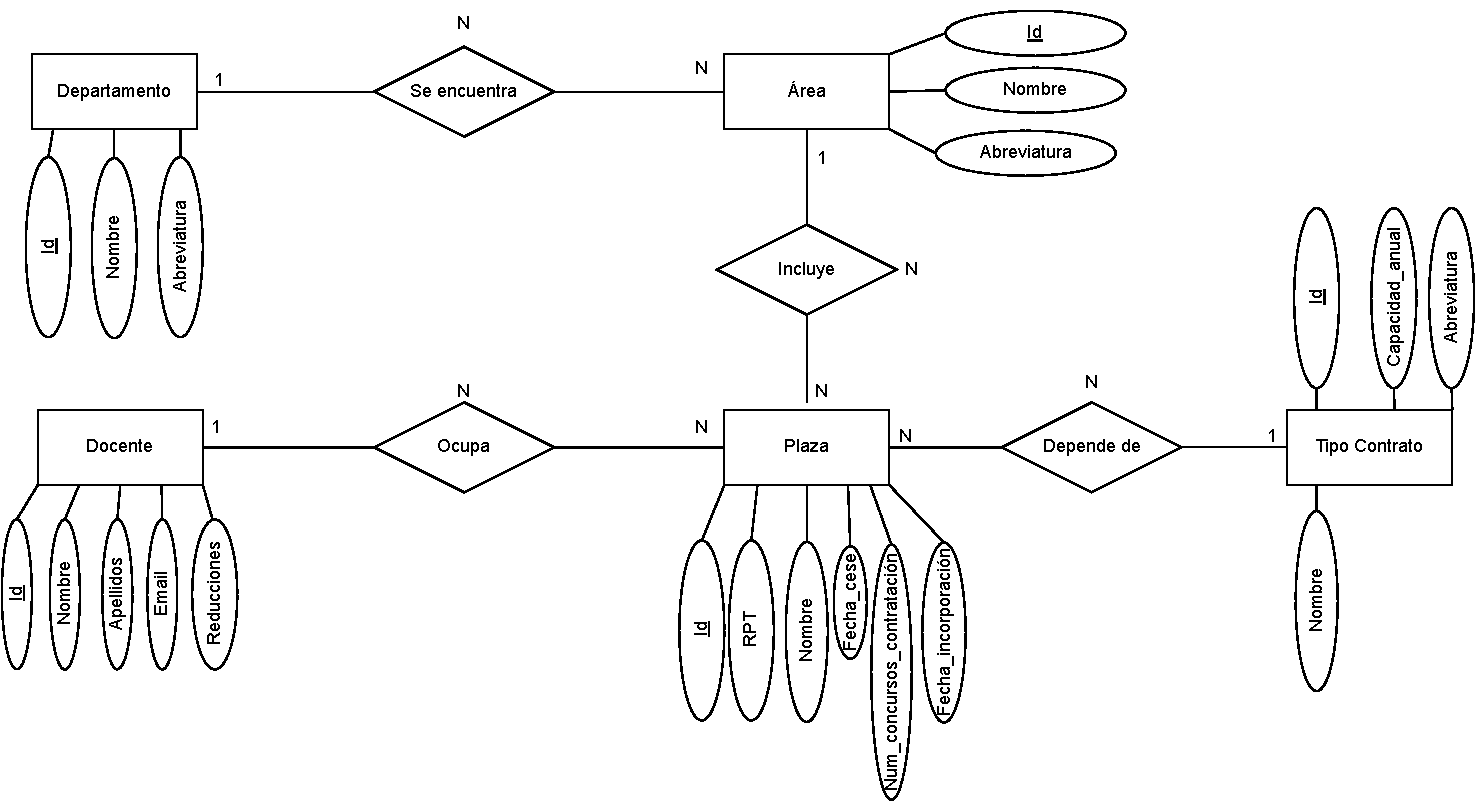
\includegraphics[scale=0.7]{../img/Anexos/Casos uso/Vistas ER/Diagrama E-R CU 2.pdf}
	\caption{Vista diagrama entidad relación para el CU-2}\label{er_cu2}
\end{figure}
\FloatBarrier

\newpage
\subsubsection{3. Asignación docente}
\begin{figure}[!h]
	\centering
	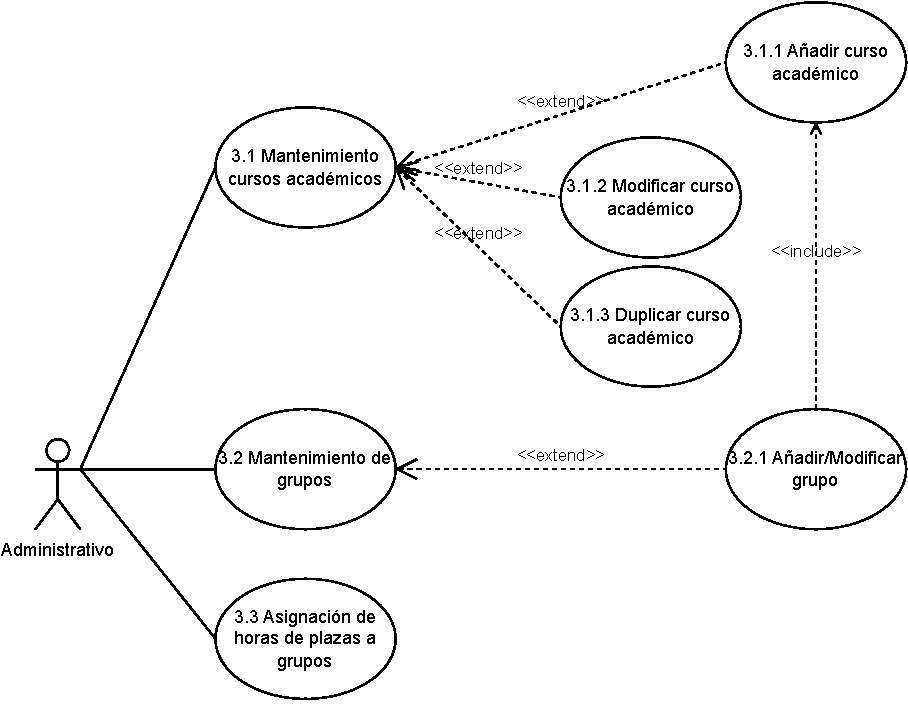
\includegraphics[scale=0.9]{../img/Anexos/Casos uso/Diagrama casos de uso 4.pdf}
	\caption{Diagrama de caso de uso - 3. Asignación docente}
\end{figure}
\FloatBarrier

\begin{table}[p]
\label{table:CU-3}
	\centering
	\begin{tabularx}{\linewidth}{ p{0.21\columnwidth} p{0.71\columnwidth} }
		\toprule
		\textbf{CU-3}    & \textbf{Asignación docente}\\
		\toprule
		\textbf{Versión}              & 1.0    \\
		\textbf{Autor}                & Ignacio Dávila García \\
		\textbf{Requisitos asociados} & \hyperref[itm:RF6]{RF-06}, \hyperref[itm:RF7]{RF-07}, \hyperref[itm:RF8]{RF-08}, \hyperref[itm:RF9]{RF-09}, \hyperref[itm:RF10]{RF-10} \\
		\textbf{Descripción}          & Un administrativo puede realizar las labores de mantenimiento de cursos y grupos, además de las asignaciones de horas de plazas a grupos \\
		\textbf{Precondición}         & Tener iniciada sesión con una cuenta con permisos administrativos \\
		\textbf{Acciones}             &
		\begin{enumerate}
			\def\labelenumi{\arabic{enumi}.}
			\tightlist
			\item Seleccionar la opción del menú <<Grupos>> para realizar el mantenimiento de los mismos.
			\item Se abre la ventana de mantenimiento de cursos.
		\end{enumerate}\\
		\textbf{Postcondición}        & El sistema lleva al usuario a la ventana de la opción pulsada. \\
		\textbf{Excepciones}          & Otras posibilidades del caso de uso son el mantenimiento de cursos académicos, que se puede realizar seleccionando la opción del menú <<Cursos>> (\hyperref[table:CU-3.1]{CU-3.1}) y la asignación de horas de una plaza a un grupo, que se puede realizar seleccionando la opción <<Horas>> (\hyperref[table:CU-3.3]{CU-3.3}). \\
		\textbf{Importancia}          & Alta \\
		\bottomrule
	\end{tabularx}
	\caption{CU-3 Asignación docente.}
\end{table}
\FloatBarrier

\begin{table}[p]
\label{table:CU-3.1}
	\centering
	\begin{tabularx}{\linewidth}{ p{0.21\columnwidth} p{0.71\columnwidth} }
		\toprule
		\textbf{CU-3.1}    & \textbf{Mantenimiento cursos académicos}\\
		\toprule
		\textbf{Versión}              & 1.0    \\
		\textbf{Autor}                & Ignacio Dávila García \\
		\textbf{Requisitos asociados} & \hyperref[itm:RF6]{RF-06} \\
		\textbf{Descripción}          & Un administrativo puede realizar el mantenimiento de los cursos académicos \\
		\textbf{Precondición}         & Realizar el~\hyperref[table:CU-3]{CU-3} \\
		\textbf{Acciones}             &
		\begin{enumerate}
			\def\labelenumi{\arabic{enumi}.}
			\tightlist
			\item Seleccionar la opción <<Cursos>> del menú principal de la web.
			\item Se abre una ventana donde aparece una tabla con los cursos creados desde donde se podrá realizar el mantenimiento.
		\end{enumerate}\\
		\textbf{Postcondición}        & Ninguna \\
		\textbf{Excepciones}          & Si se pulsa sobre el botón <<Nuevo>>, se accede a la creación de un curso (\hyperref[table:CU-3.1.1]{CU-3.1.1}), si se pulsa sobre el botón <<Modificar>> de un curso de la lista, se accede a la ventana de modificación (\hyperref[table:CU-3.1.2]{CU-3.1.2}), si se pulsa sobre el botón <<Modificar Año>> de un curso de la lista, se accede a la ventana de modificación del campo año de inicio, si se pulsa sobre el botón <<Eliminar>> de un curso el sistema pregunta si está seguro, y al pulsar en <<Sí>>, este se elimina produciendo un borrado en cascada de sus relaciones con asignaturas y grupos. Por último, si se pulsa sobre <<Duplicar>>, se duplica el curso junto a todas sus vinculaciones  (\hyperref[table:CU-3.1.3]{CU-3.1.3})\\
		\textbf{Importancia}          & Alta \\
		\bottomrule
	\end{tabularx}
	\caption{CU-3.1 Mantenimiento cursos académicos.}
\end{table}
\FloatBarrier

\begin{table}[p]
\label{table:CU-3.1.1}
	\centering
	\begin{tabularx}{\linewidth}{ p{0.21\columnwidth} p{0.71\columnwidth} }
		\toprule
		\textbf{CU-3.1.1}    & \textbf{Añadir curso académico}\\
		\toprule
		\textbf{Versión}              & 1.0    \\
		\textbf{Autor}                & Ignacio Dávila García \\
		\textbf{Requisitos asociados} & \hyperref[itm:RF3]{RF-03}, \hyperref[itm:RF6]{RF-06} \\
		\textbf{Descripción}          & Un administrativo añade un curso académico \\
		\textbf{Precondición}         & Realizar el~\hyperref[table:CU-3.1]{CU-3.1} \\
		\textbf{Acciones}             &
		\begin{enumerate}
			\def\labelenumi{\arabic{enumi}.}
			\tightlist
			\item Se abre una ventana con un formulario. El formulario contiene un campo para indicar el año de comienzo del curso.
			\item Pulsar en el botón <<Siguiente>>
			\item Se abre una ventana que contiene una tabla con las asignaturas existentes desde donde se podrán seleccionar las deseadas. También contiene tres bloques para las diferentes modalidades donde se podrá indicar el número de alumnos previstos, el número de grupos de teoría y el número de grupos de práctica que se deben crear para las asignaturas seleccionadas.
			\item Pulsar en el botón <<Añadir>>
			\item Aparece la misma pantalla con los campos limpios para poder añadir más asignaturas y grupos.
		\end{enumerate}\\
		\textbf{Postcondición}        & El curso se crea junto a las asignaturas y grupos elegidos. \\
		\textbf{Excepciones}          & Se dejan campos vacíos o se introducen datos con un formato incorrecto. \\
		\textbf{Importancia}          & Alta \\
		\bottomrule
	\end{tabularx}
	\caption{CU-3.1.1 Añadir curso académico.}
\end{table}
\FloatBarrier

\begin{table}[p]
\label{table:CU-3.1.2}
	\centering
	\begin{tabularx}{\linewidth}{ p{0.21\columnwidth} p{0.71\columnwidth} }
		\toprule
		\textbf{CU-3.1.2}    & \textbf{Modificar curso académico}\\
		\toprule
		\textbf{Versión}              & 1.0    \\
		\textbf{Autor}                & Ignacio Dávila García \\
		\textbf{Requisitos asociados} & \hyperref[itm:RF3]{RF-03}, \hyperref[itm:RF6]{RF-06} \\
		\textbf{Descripción}          & Un administrativo modifica un curso académico \\
		\textbf{Precondición}         & Realizar el~\hyperref[table:CU-3.1]{CU-3.1} \\
		\textbf{Acciones}             &
		\begin{enumerate}
			\def\labelenumi{\arabic{enumi}.}
			\tightlist
			\item Se abre una ventana con el listado de asignaturas del curso. Desde esa ventana se pueden añadir nuevas asignaturas al curso pulsando sobre el botón <<Añadir asignaturas>>.
			\item Al pulsar sobre <<Añadir asignaturas>> se abre una ventana flotante desde la que se pueden seleccionar las asignaturas e indicar el número de alumnos previstos y el número de grupos de teoría y práctica a crear para cada modalidad. 
			\item Pulsar sobre el botón <<Añadir>>.
			\item La ventana se cierra y se puede ver en la tabla como las nuevas asignaturas aparecen vinculadas al curso.
		\end{enumerate}\\
		\textbf{Postcondición}        & El curso se modifica y el sistema permanece en la ventana de modificación del curso desde donde se pueden ver los cambios realizados. \\
		\textbf{Excepciones}          & Si se pulsa sobre el botón <<Quitar del curso>> de una de las asignaturas, el sistema pregunta si está seguro de la eliminación, y al pulsar en la opción <<Sí>>, la asignatura desaparece del listado y se produce un borrado en cascada de sus grupos. Si se pulsa sobre el botón <<Editar grupos>> de una de las asignaturas se abre una ventana desde donde realizar la modificación de los grupos de la asignatura para ese curso. (\hyperref[table:CU-3.2.1]{CU-3.2.1}) \\
		\textbf{Importancia}          & Alta \\
		\bottomrule
	\end{tabularx}
	\caption{CU-3.1.2 Modificar curso académico.}
\end{table}
\FloatBarrier

\begin{table}[p]
\label{table:CU-3.1.3}
	\centering
	\begin{tabularx}{\linewidth}{ p{0.21\columnwidth} p{0.71\columnwidth} }
		\toprule
		\textbf{CU-3.1.3}    & \textbf{Duplicar curso académico}\\
		\toprule
		\textbf{Versión}              & 1.0    \\
		\textbf{Autor}                & Ignacio Dávila García \\
		\textbf{Requisitos asociados} & \hyperref[itm:RF6]{RF-06} \\
		\textbf{Descripción}          & Un administrativo duplica un curso académico con toda la información asociada \\
		\textbf{Precondición}         & Realizar el~\hyperref[table:CU-3.1]{CU-3.1} \\
		\textbf{Acciones}             &
		\begin{enumerate}
			\def\labelenumi{\arabic{enumi}.}
			\tightlist
			\item Se abre una ventana modal de confirmación donde se pregunta si está seguro de duplicar el curso académico.
			\item Pulsar en la opción <<Sí>>.
		\end{enumerate}\\
		\textbf{Postcondición}        & El curso y todas sus asociaciones se duplican y el sistema permanece en la ventana de mantenimiento de cursos desde donde se puede ver como el nuevo curso se ha creado. El nuevo curso se crea con un año más en el campo año de inicio que el último existente. \\
		\textbf{Excepciones}          & Ninguna \\
		\textbf{Importancia}          & Alta \\
		\bottomrule
	\end{tabularx}
	\caption{CU-3.1.3 Duplicar curso académico.}
\end{table}
\FloatBarrier

\begin{table}[p]
\label{table:CU-3.2}
	\centering
	\begin{tabularx}{\linewidth}{ p{0.21\columnwidth} p{0.71\columnwidth} }
		\toprule
		\textbf{CU-3.2}    & \textbf{Mantenimiento de grupos}\\
		\toprule
		\textbf{Versión}              & 1.0    \\
		\textbf{Autor}                & Ignacio Dávila García \\
		\textbf{Requisitos asociados} & \hyperref[itm:RF3]{RF-03} \\
		\textbf{Descripción}          & Un administrativo puede realizar el mantenimiento de grupos \\
		\textbf{Precondición}         & Realizar el~\hyperref[table:CU-3]{CU-3} \\
		\textbf{Acciones}             &
		\begin{enumerate}
			\def\labelenumi{\arabic{enumi}.}
			\tightlist
			\item Se abre una ventana donde aparece un seleccionador de curso, con el último curso seleccionado por defecto. También aparece una tabla con todas las asignaturas del curso seleccionado junto al número de grupos de cada tipo que tienen vinculados.
		\end{enumerate}\\
		\textbf{Postcondición}        & Ninguna \\
		\textbf{Excepciones}          & Si se pulsa sobre el botón <<Gestionar grupos>> de uno de los registros de la tabla se accede a una ventana con la información de la asignatura y sus grupos. Desde esta ventana se pueden crear, modificar o eliminar grupos para esa asignatura. (\hyperref[table:CU-3.2.1]{CU-3.2.1}) \\
		\textbf{Importancia}          & Alta \\
		\bottomrule
	\end{tabularx}
	\caption{CU-3.2 Mantenimiento de grupos.}
\end{table}
\FloatBarrier

\begin{table}[p]
\label{table:CU-3.2.1}
	\centering
	\begin{tabularx}{\linewidth}{ p{0.21\columnwidth} p{0.71\columnwidth} }
		\toprule
		\textbf{CU-3.2.1}    & \textbf{Añadir/Modificar grupo}\\
		\toprule
		\textbf{Versión}              & 1.0    \\
		\textbf{Autor}                & Ignacio Dávila García \\
		\textbf{Requisitos asociados} & \hyperref[itm:RF3]{RF-03}, \hyperref[itm:RF13]{RF-13} \\
		\textbf{Descripción}          & Un administrativo añade o modifica los grupos de una asignatura \\
		\textbf{Precondición}         & Realizar el~\hyperref[table:CU-3.2]{CU-3.2} \\
		\textbf{Acciones}             &
		\begin{enumerate}
			\def\labelenumi{\arabic{enumi}.}
			\tightlist
			\item Pulsar sobre el botón <<Gestionar grupos>> de una de las asignaturas de la tabla.
			\item Se abre una nueva ventana con la información de la asignatura y un listado con los grupos que tiene vinculados.
			\item Pulsar sobre el botón <<Añadir grupo>>.
			\item Se abre una ventana flotante con un formulario que contiene los campos de la tabla <<Grupo>> de la figura \ref{er_cu3}.
			\item Completar los campos y pulsar en el botón <<Añadir>>
		\end{enumerate}\\
		\textbf{Postcondición}        & El grupo se crea y queda vinculado a la asignatura. El usuario termina el caso de uso en la ventana que contiene los grupos de la asignatura. \\
		\textbf{Excepciones}          & Se dejan campos vacíos o se introducen datos con un formato incorrecto. Otra forma de finalizar el caso de uso es la modificación o eliminación. En el primer caso, se pulsa sobre el botón <<Modificar>> de un grupo de la tabla y se accede al mismo formulario de creación, pero con los campos rellenos. Si se pulsa en el botón <<Modificar>> la información del grupo queda actualizada. Por último, para el caso de eliminar, se pulsa sobre el botón <<Eliminar>> de un grupo de la tabla, el sistema pregunta si está seguro, y al pulsar en <<Sí>>, este se elimina. \\
		\textbf{Importancia}          & Alta \\
		\bottomrule
	\end{tabularx}
	\caption{CU-3.2.1 Añadir/Modificar grupo.}
\end{table}
\FloatBarrier

\begin{table}[p]
\label{table:CU-3.3}
	\centering
	\begin{tabularx}{\linewidth}{ p{0.21\columnwidth} p{0.71\columnwidth} }
		\toprule
		\textbf{CU-3.3}    & \textbf{Asignación de horas de plazas a grupos}\\
		\toprule
		\textbf{Versión}              & 1.0    \\
		\textbf{Autor}                & Ignacio Dávila García \\
		\textbf{Requisitos asociados} & \hyperref[itm:RF11]{RF-11} \\
		\textbf{Descripción}          & Un administrativo puede asignar horas de una plaza a un grupo durante un curso académico \\
		\textbf{Precondición}         & Realizar el~\hyperref[table:CU-3]{CU-3} \\
		\textbf{Acciones}             &
		\begin{enumerate}
			\def\labelenumi{\arabic{enumi}.}
			\tightlist
			\item Se abre una ventana donde aparece un seleccionador de curso, con el último curso seleccionado por defecto. También aparece una tabla con todos los grupos del curso y las plazas/docentes que tienen vinculados.
			\item Pulsar sobre el botón <<Editar>> de una de las filas de la tabla.
			\item Se abre una nueva ventana con la información del grupo y un listado con las plazas vinculadas.
			\item Para vincular una nueva plaza pulsar sobre el botón <<Añadir plaza>>.
			\item Se abre una ventana flotante donde se puede buscar por el nombre de la plaza o del docente que se quiere vincular.
			\item Pulsar sobre la plaza/docente a vincular e indicar en el campo horas el número de horas asignadas al grupo.
			\item Pulsar sobre el botón <<Vincular>>.
		\end{enumerate}\\
		\textbf{Postcondición}        & La plaza seleccionada se vincula al grupo con el número de horas indicado. El sistema permanece en la ventana del grupo donde aparecen las plazas asignadas. \\
		\textbf{Excepciones}          & Otra forma de finalizar el caso de uso es desvincular una plaza de un grupo. Para ello se pulsa en el botón <<Eliminar>> del listado de plazas del grupo. Aparece una ventana modal que pregunta si está seguro de la eliminación y, al pulsar en <<Sí>>, desaparece la vinculación de la plaza al grupo.
		Finalmente, las horas que tiene asignadas una plaza/docente se pueden modificar. Para ello, se cambia el número de horas de la plaza desde la tabla (columna <<Horas anuales>>) y para guardar los cambios se pulsa en el botón <<Modificar>>. \\
		\textbf{Importancia}          & Alta \\
		\bottomrule
	\end{tabularx}
	\caption{CU-3.3 Asignación de horas de plazas a grupos.}
\end{table}
\FloatBarrier

\begin{figure}[!h]
	\centering
	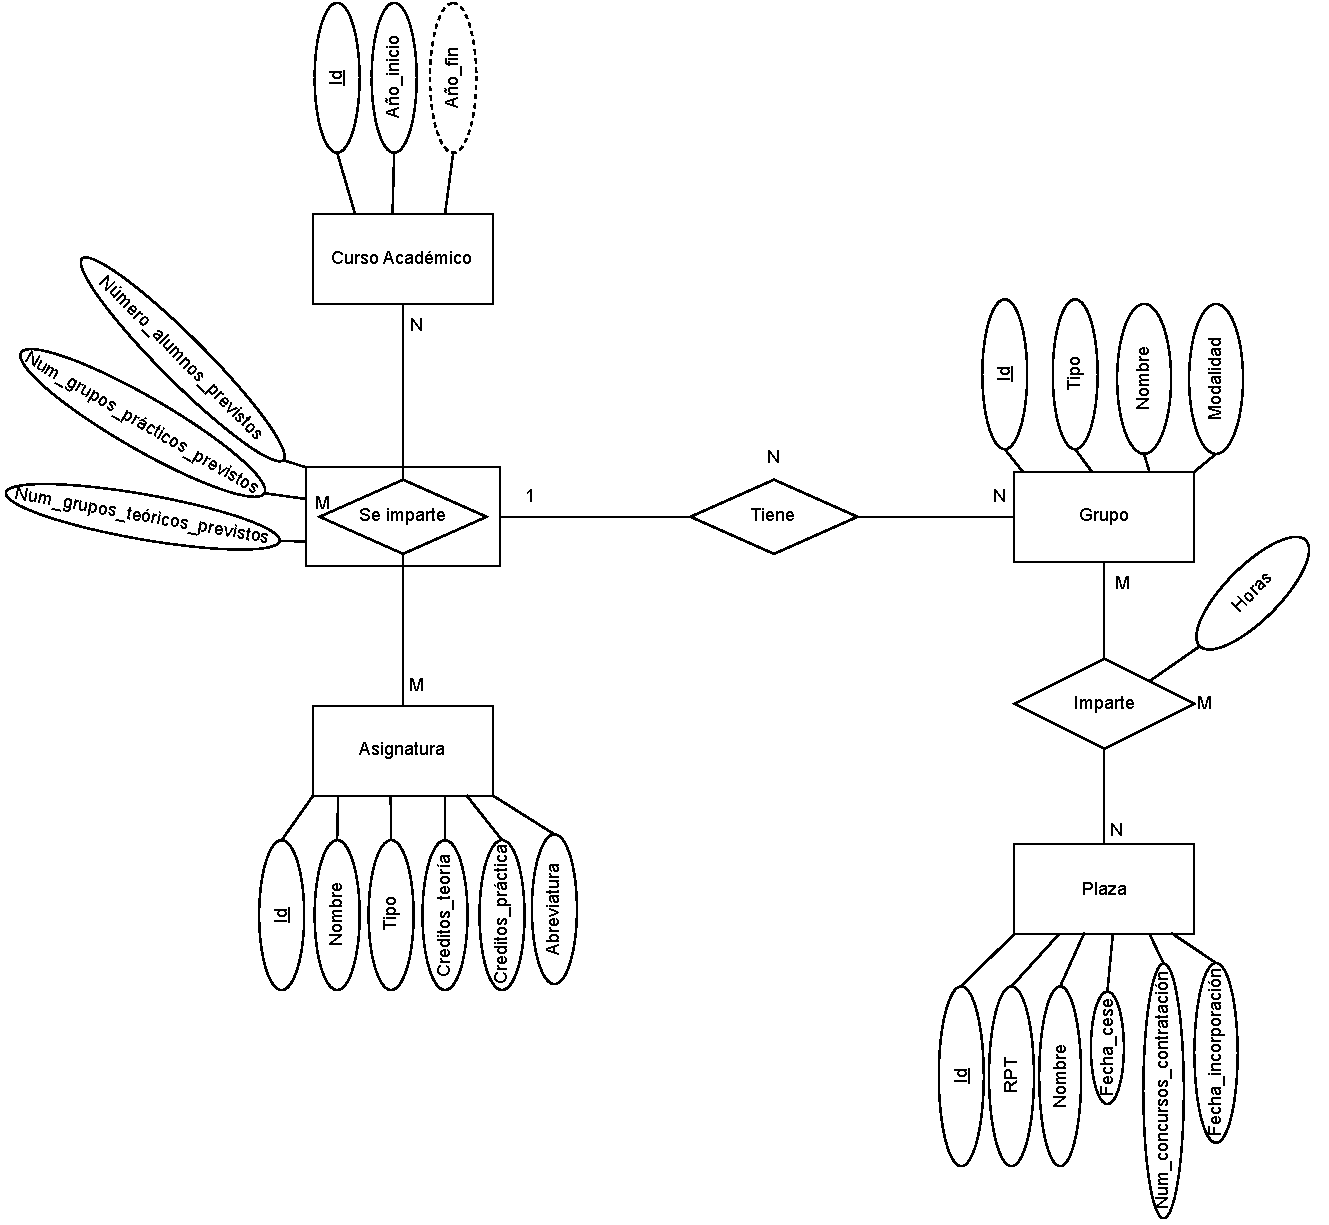
\includegraphics[scale=0.8]{../img/Anexos/Casos uso/Vistas ER/Diagrama E-R CU 3.pdf}
	\caption{Vista diagrama entidad relación para el CU-3}\label{er_cu3}
\end{figure}
\FloatBarrier

\newpage
\subsection{Prototipos de vistas de los casos de uso}
\begin{itemize}
	\item \textbf{CU-1.} Mantenimiento académico.
	\begin{itemize}
		\item \textbf{CU-1.1} Mantenimiento de centros. Ver figura~\ref{F-CU1.1}
		\begin{figure}[!h]
		\centering
		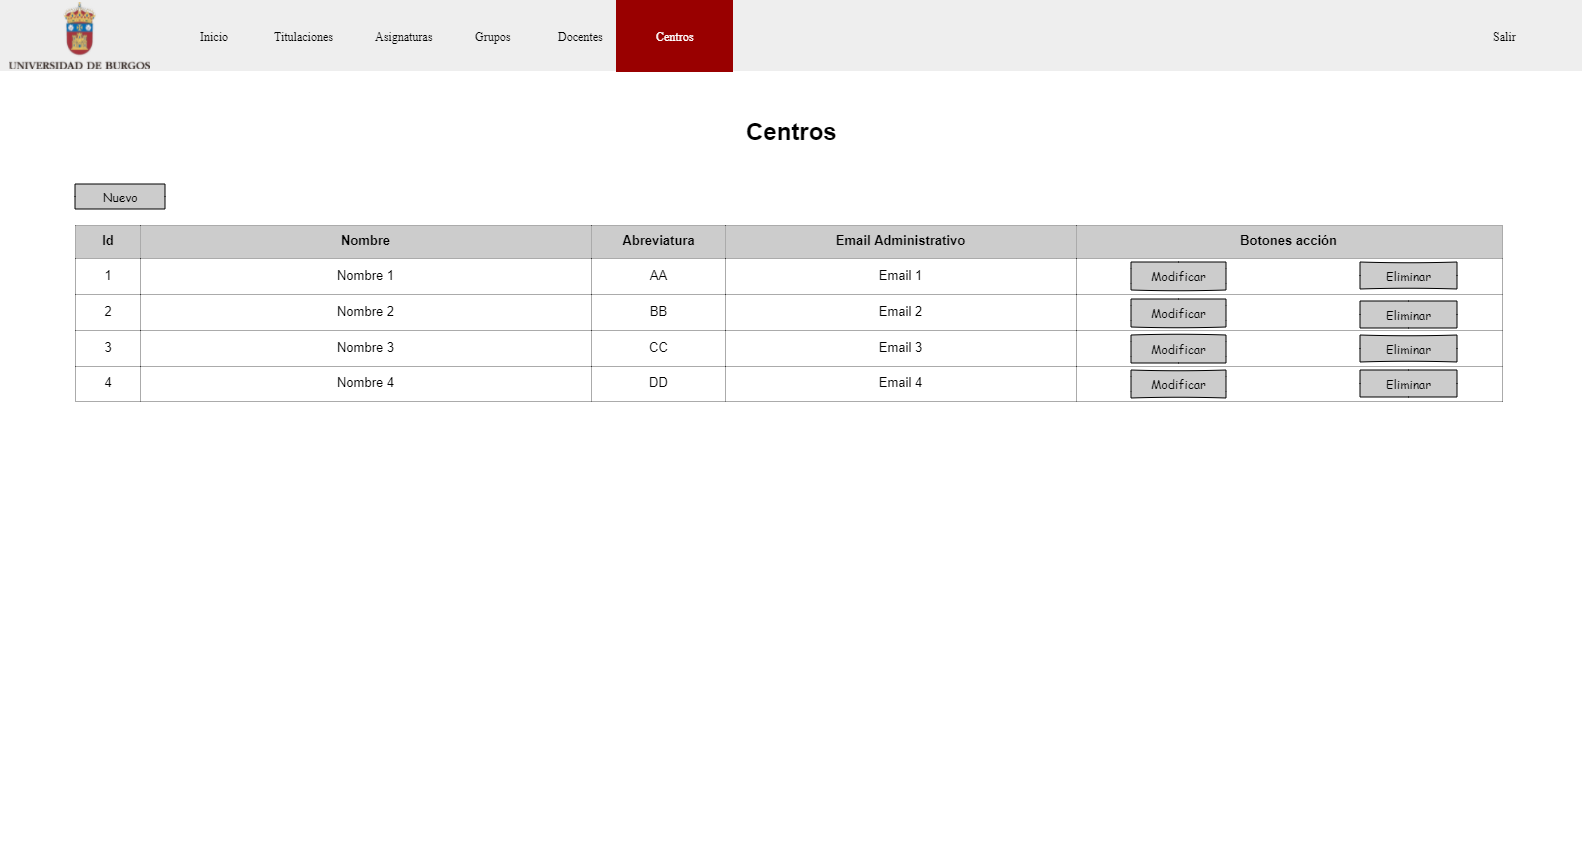
\includegraphics[width=\textwidth]{../img/Anexos/Vistas/centros.png}
		\caption{Mantenimiento de centros}\label{F-CU1.1}
		\end{figure}
		\FloatBarrier
		\item \textbf{CU-1.1.1} Añadir/Modificar centros. Ver figura~\ref{F-CU1.1.1}
		\begin{figure}[!h]
		\centering
		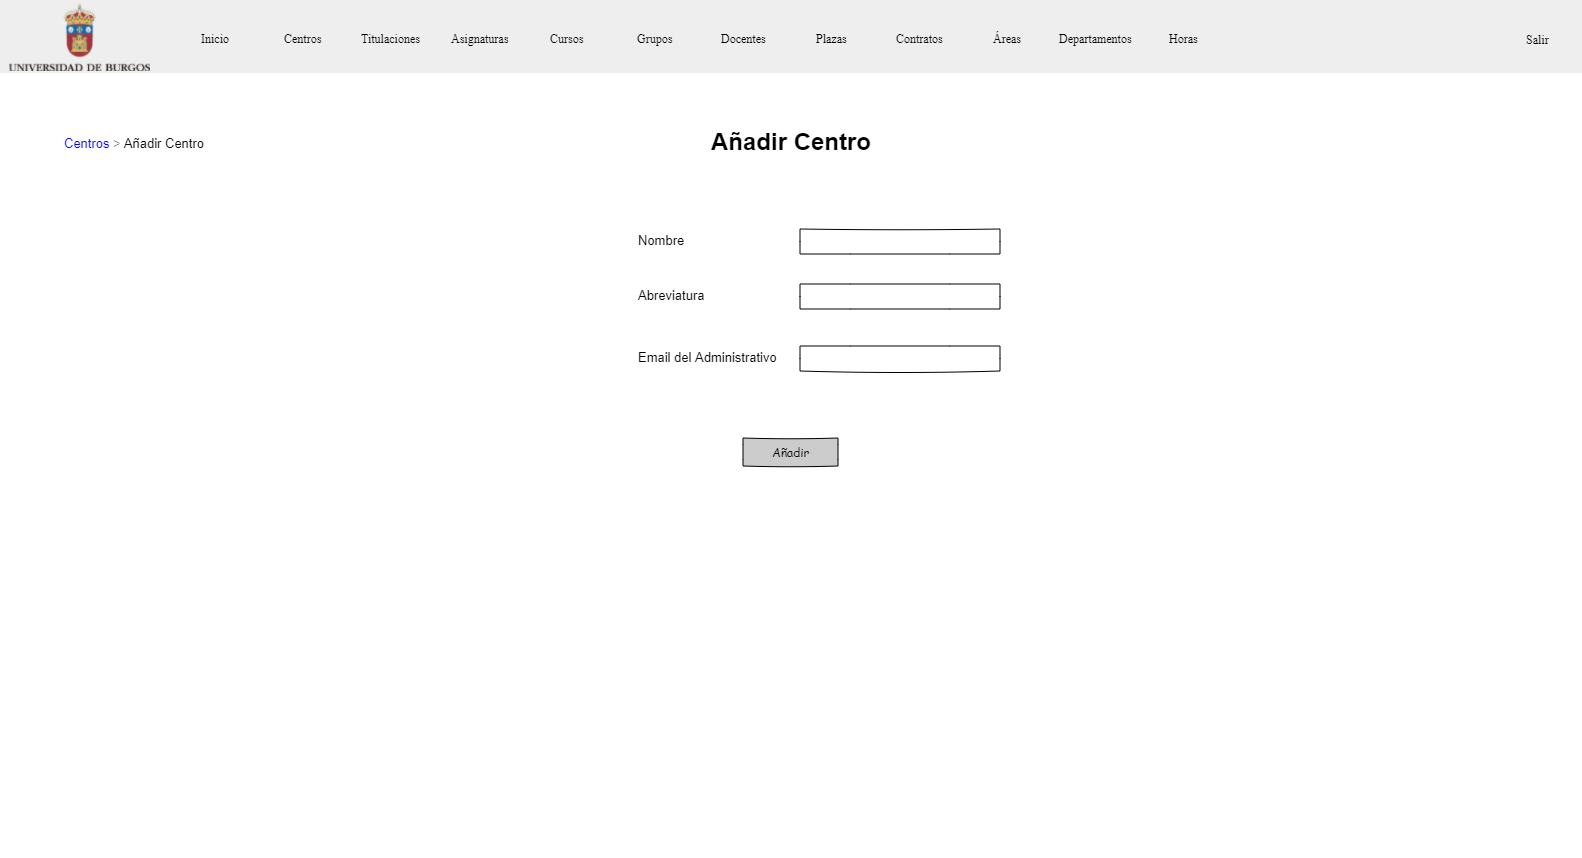
\includegraphics[width=\textwidth]{../img/Anexos/Vistas/add_centro.png}
		\caption{Añadir/Modificar centros}\label{F-CU1.1.1}
		\end{figure}
		\FloatBarrier
\newpage
		\item \textbf{CU-1.2} Mantenimiento de titulaciones. Ver figura~\ref{F-CU1.2}
		\begin{figure}[!h]
		\centering
		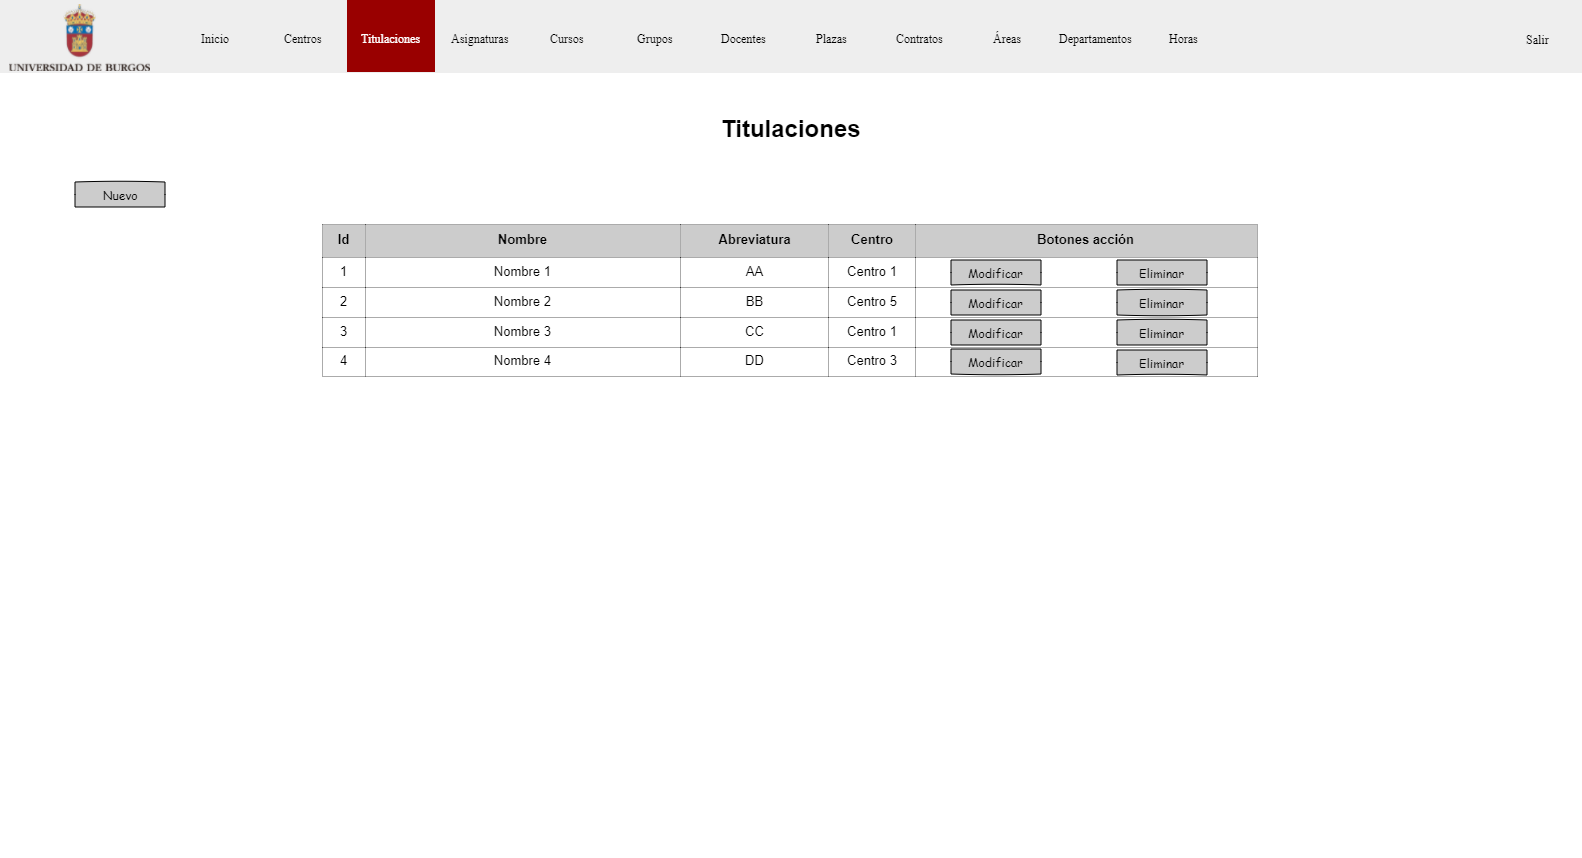
\includegraphics[width=\textwidth]{../img/Anexos/Vistas/titulaciones.png}
		\caption{Mantenimiento de titulaciones}\label{F-CU1.2}
		\end{figure}
		\FloatBarrier
		\item \textbf{CU-1.2.1} Añadir/Modificar titulaciones. Ver figura~\ref{F-CU1.2.1}
		\begin{figure}[!h]
		\centering
		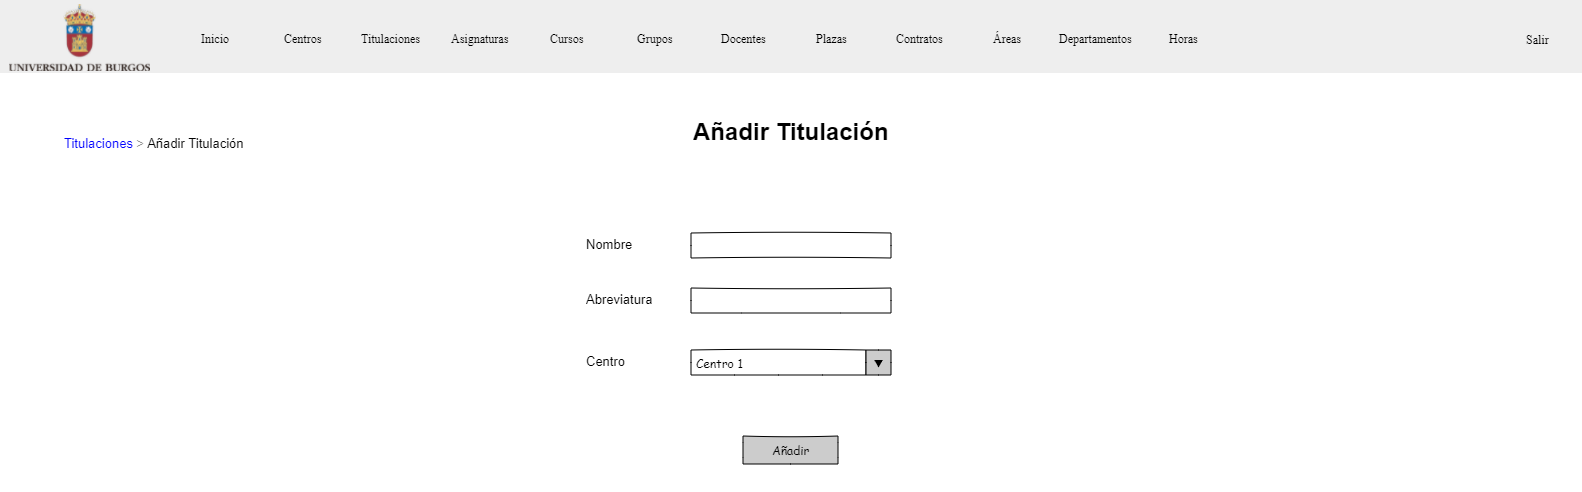
\includegraphics[width=\textwidth]{../img/Anexos/Vistas/add_titulacion.png}
		\caption{Añadir/Modificar titulaciones}\label{F-CU1.2.1}
		\end{figure}
		\FloatBarrier
\newpage
		\item \textbf{CU-1.3} Mantenimiento de asignaturas. Ver figura~\ref{F-CU1.3}
		\begin{figure}[!h]
		\centering
		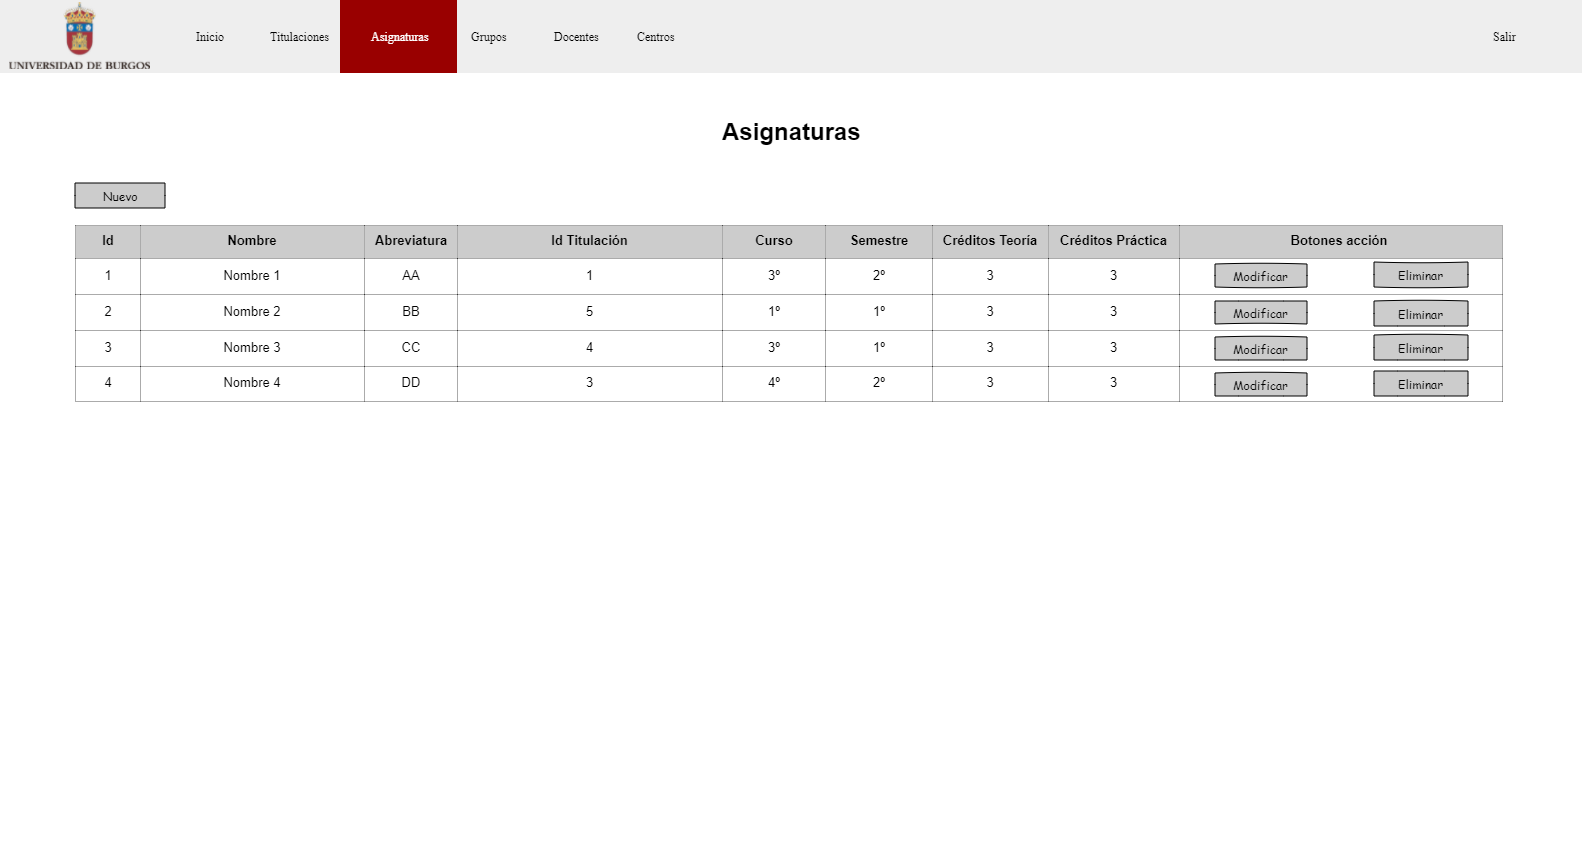
\includegraphics[width=\textwidth]{../img/Anexos/Vistas/asignaturas.png}
		\caption{Mantenimiento de asignaturas}\label{F-CU1.3}
		\end{figure}
		\FloatBarrier
		\item \textbf{CU-1.3.1} Añadir/Modificar asignaturas. Ver figura~\ref{F-CU1.3.1}
		\begin{figure}[!h]
		\centering
		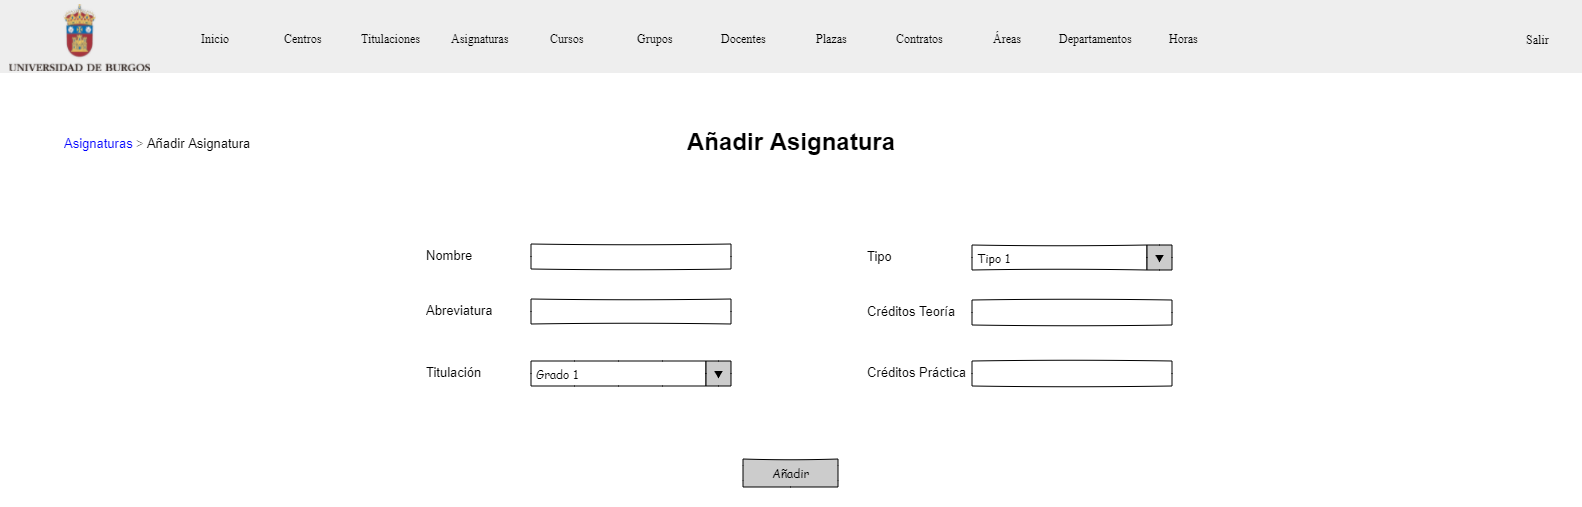
\includegraphics[width=\textwidth]{../img/Anexos/Vistas/add_asignatura.png}
		\caption{Añadir/Modificar asignaturas}\label{F-CU1.3.1}
		\end{figure}
		\FloatBarrier
	\end{itemize}
	
\newpage	
	\item \textbf{CU-2.} Mantenimiento de profesorado.
	\begin{itemize}
		\item \textbf{CU-2.1} Mantenimiento de departamentos. Ver figura~\ref{F-CU2.1}
		\begin{figure}[!h]
		\centering
		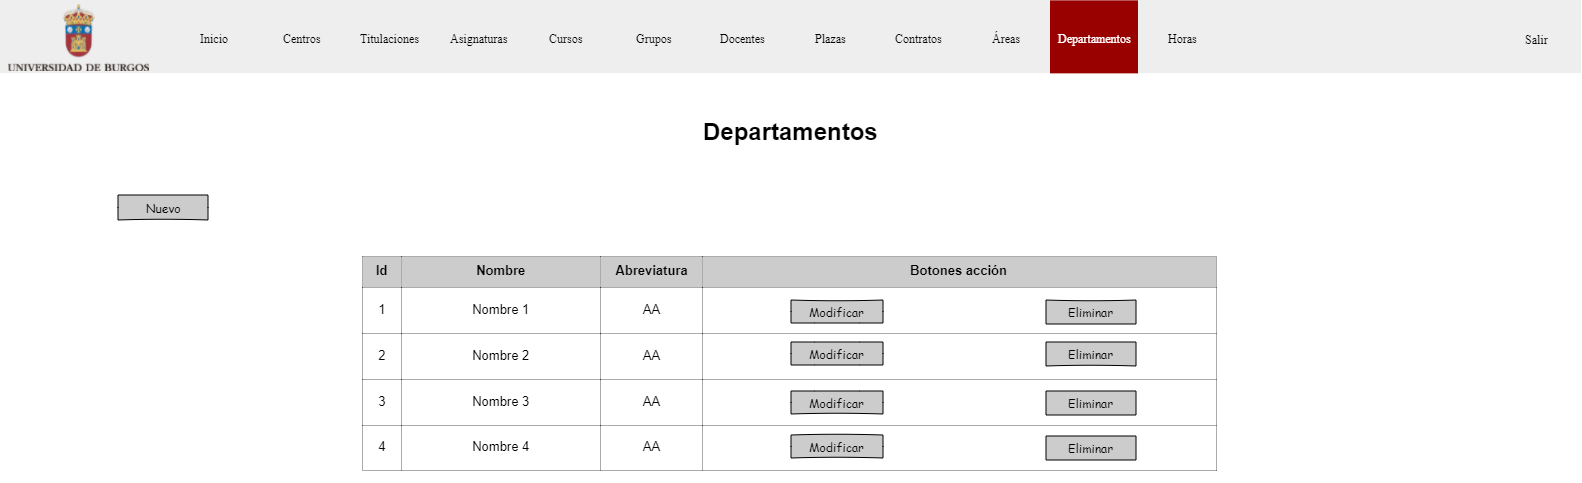
\includegraphics[width=\textwidth]{../img/Anexos/Vistas/departamentos.png}
		\caption{Mantenimiento de departamentos}\label{F-CU2.1}
		\end{figure}
		\FloatBarrier
		\item \textbf{CU-2.1.1} Añadir/Modificar departamentos. Ver figura~\ref{F-CU2.1.1}
		\begin{figure}[!h]
		\centering
		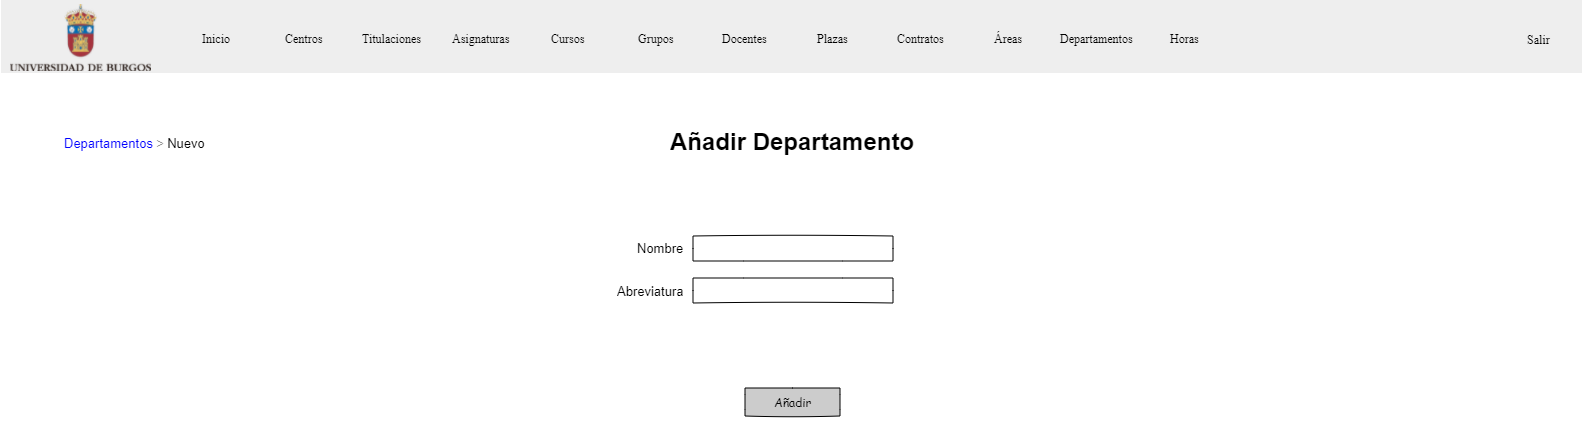
\includegraphics[width=\textwidth]{../img/Anexos/Vistas/add_departamento.png}
		\caption{Añadir/Modificar departamentos}\label{F-CU2.1.1}
		\end{figure}
		\FloatBarrier
\newpage
		\item \textbf{CU-2.2} Mantenimiento de áreas. Ver figura~\ref{F-CU2.2}
		\begin{figure}[!h]
		\centering
		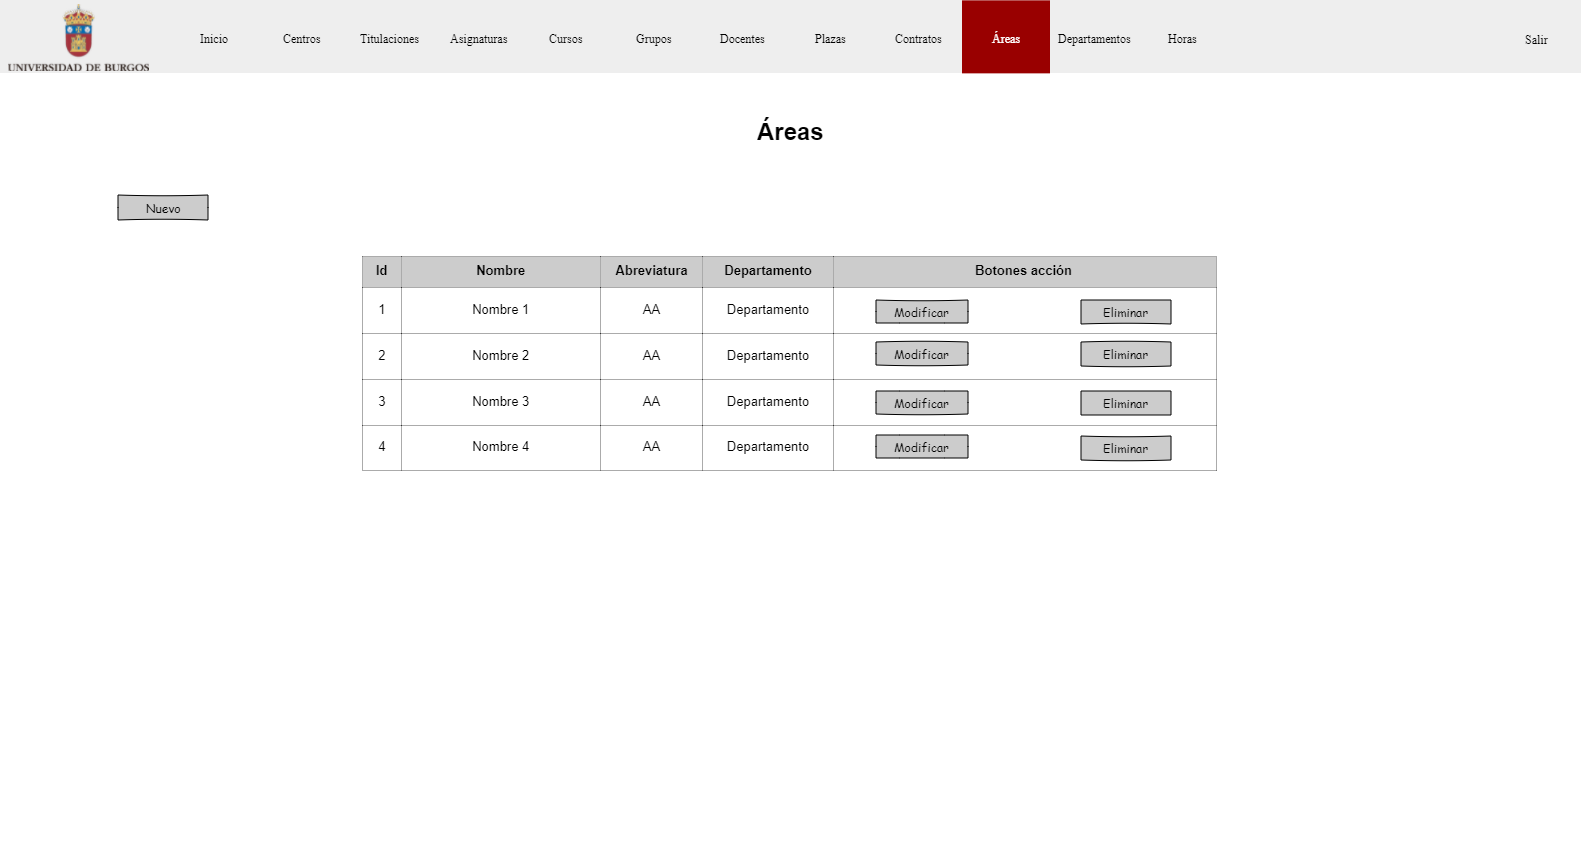
\includegraphics[width=\textwidth]{../img/Anexos/Vistas/areas.png}
		\caption{Mantenimiento de áreas}\label{F-CU2.2}
		\end{figure}
		\FloatBarrier
		\item \textbf{CU-2.2.1} Añadir/Modificar áreas. Ver figura~\ref{F-CU2.2.1}
		\begin{figure}[!h]
		\centering
		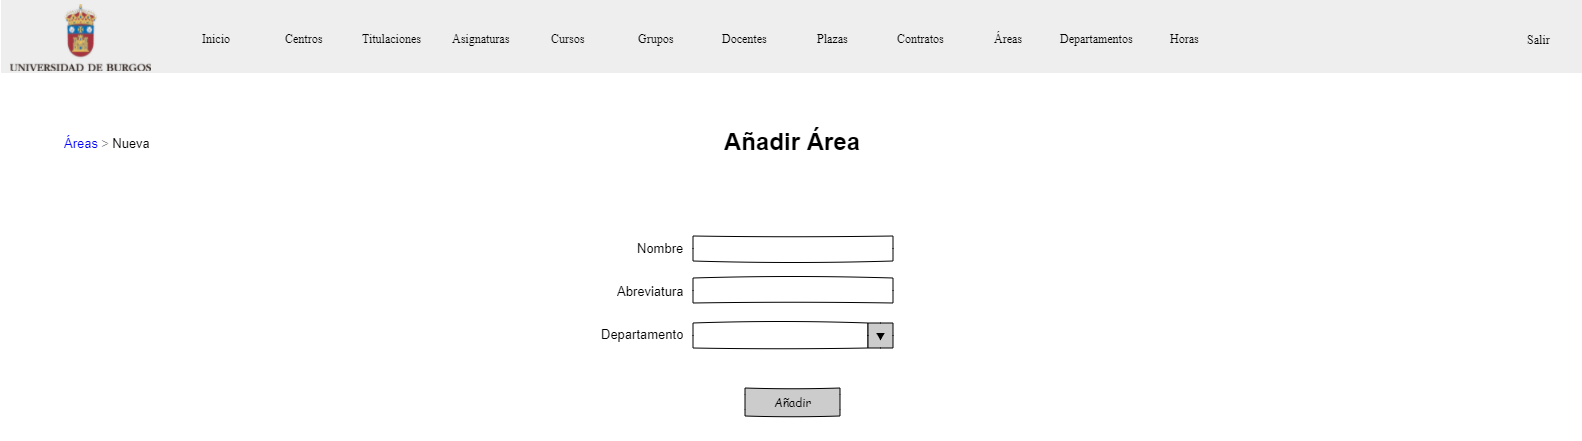
\includegraphics[width=\textwidth]{../img/Anexos/Vistas/add_area.png}
		\caption{Añadir/Modificar áreas}\label{F-CU2.2.1}
		\end{figure}
		\FloatBarrier
		\item \textbf{CU-2.3} Mantenimiento de docentes. Ver figura~\ref{F-CU2.3}
		\begin{figure}[!h]
		\centering
		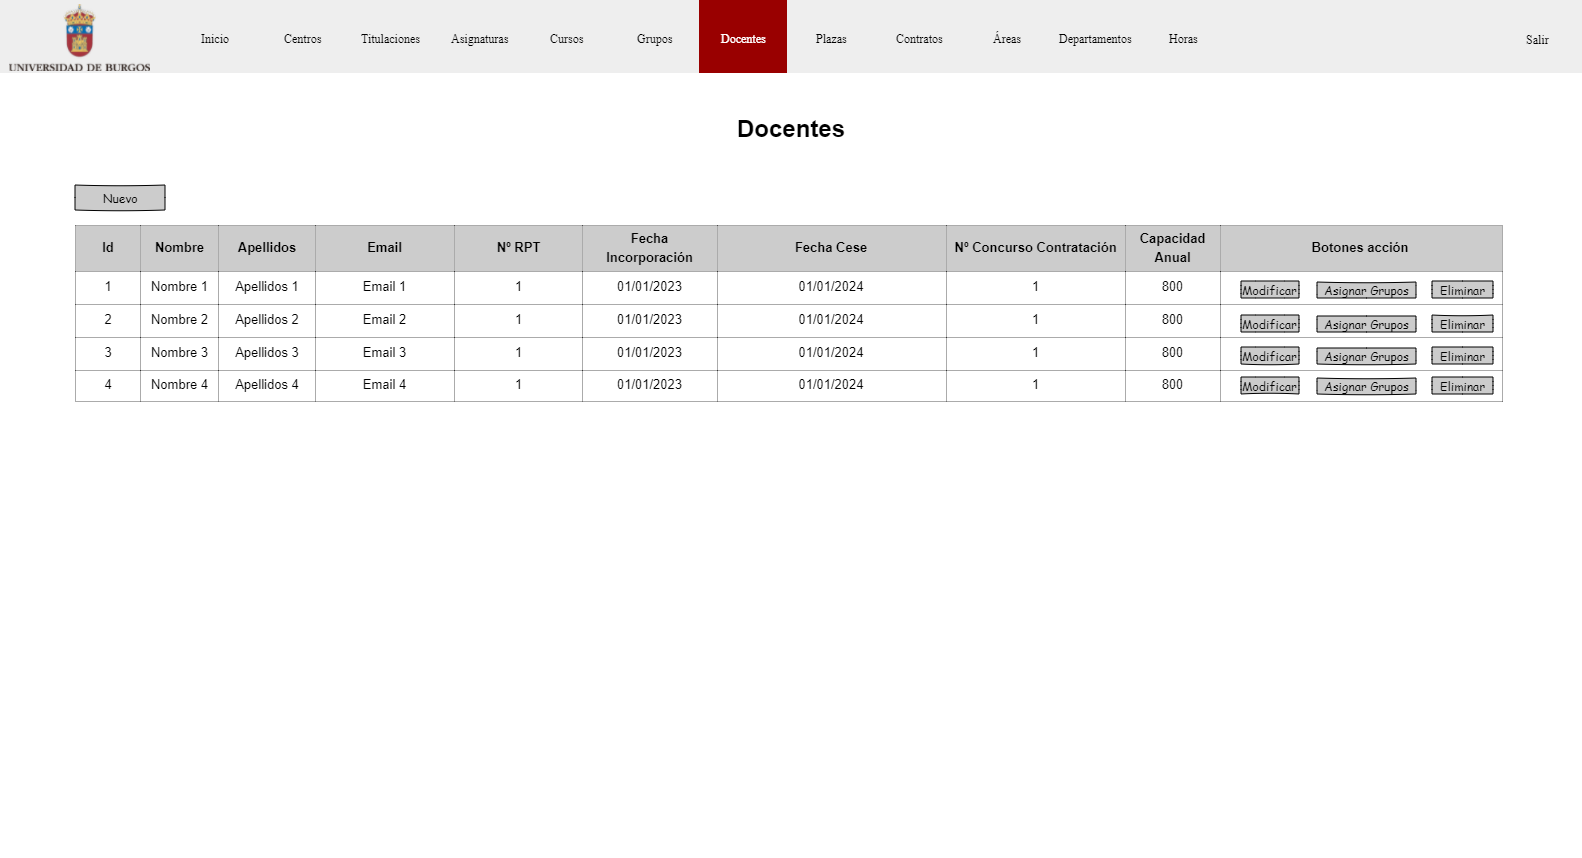
\includegraphics[width=\textwidth]{../img/Anexos/Vistas/docentes.png}
		\caption{Mantenimiento de docentes}\label{F-CU2.3}
		\end{figure}
		\FloatBarrier
\newpage
		\item \textbf{CU-2.3.1} Añadir/Modificar docentes. Ver figura~\ref{F-CU2.3.1}
		\begin{figure}[!h]
		\centering
		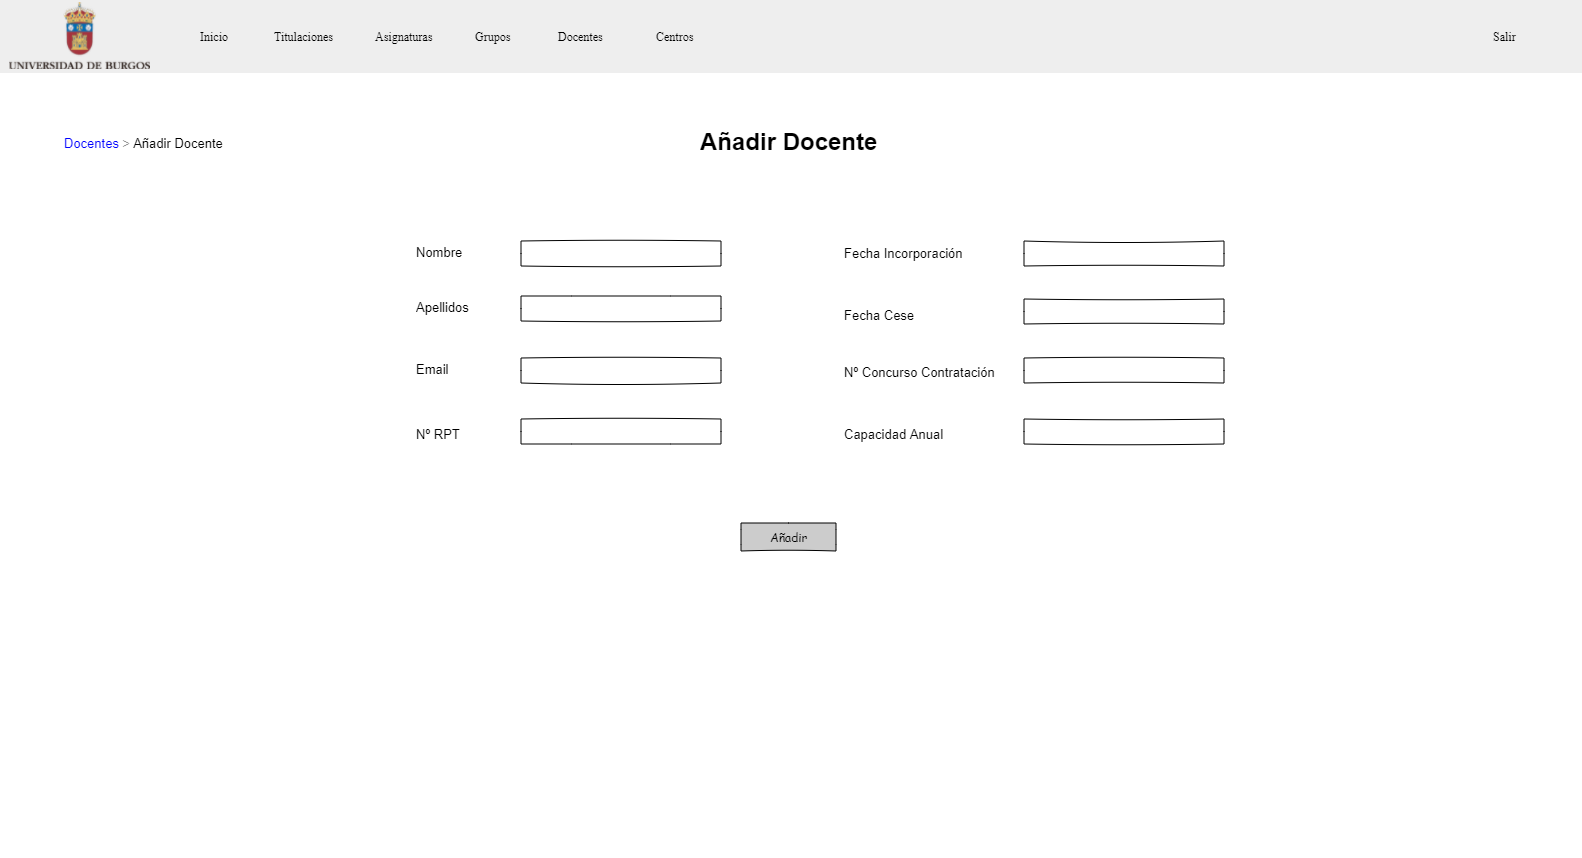
\includegraphics[width=\textwidth]{../img/Anexos/Vistas/add_docente.png}
		\caption{Añadir/Modificar docentes}\label{F-CU2.3.1}
		\end{figure}
		\FloatBarrier
		\item \textbf{CU-2.4} Mantenimiento de tipos de contrato. Ver figura~\ref{F-CU2.4}
		\begin{figure}[!h]
		\centering
		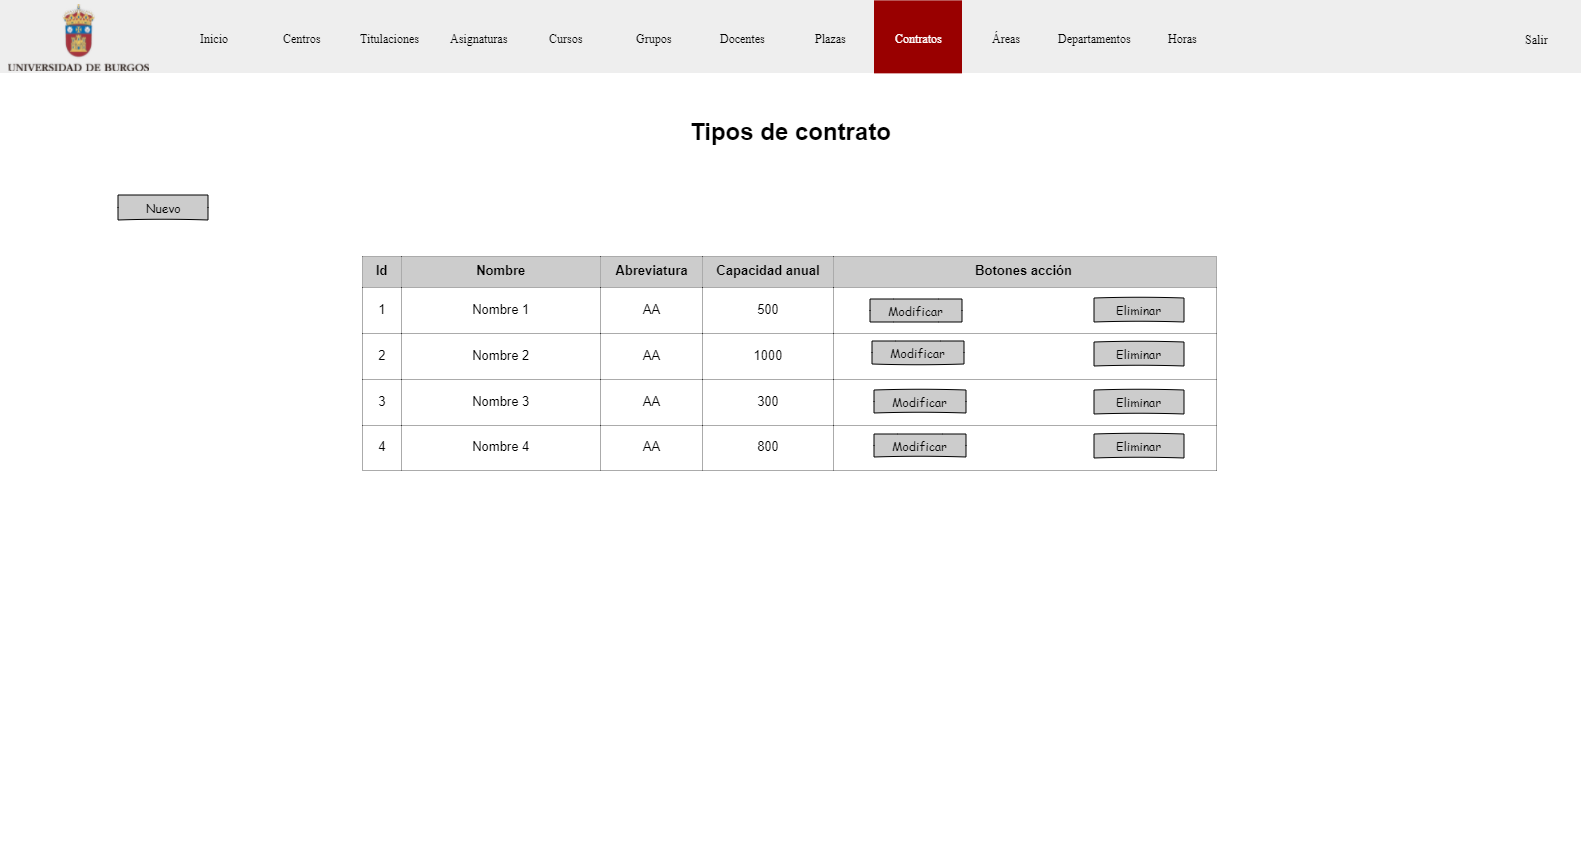
\includegraphics[width=\textwidth]{../img/Anexos/Vistas/contratos.png}
		\caption{Mantenimiento de tipos de contrato}\label{F-CU2.4}
		\end{figure}
		\FloatBarrier
\newpage
		\item \textbf{CU-2.4.1} Añadir/Modificar tipos de contrato. Ver figura~\ref{F-CU2.4.1}
		\begin{figure}[!h]
		\centering
		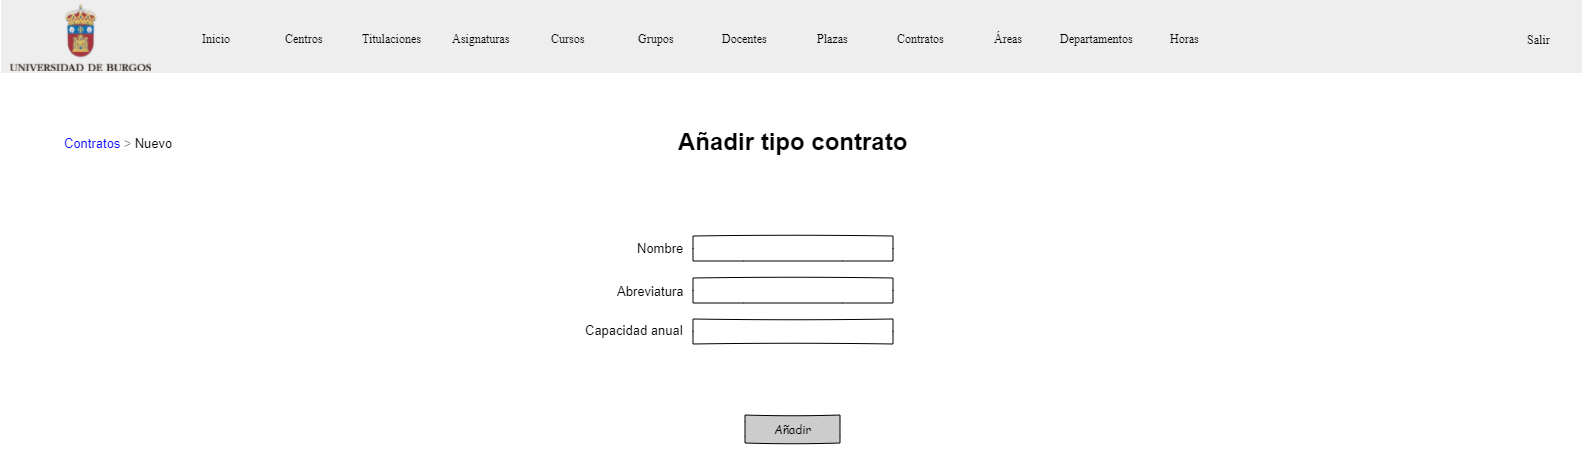
\includegraphics[width=\textwidth]{../img/Anexos/Vistas/add_contrato.png}
		\caption{Añadir/Modificar tipos de contrato}\label{F-CU2.4.1}
		\end{figure}
		\FloatBarrier
		\item \textbf{CU-2.5} Mantenimiento de plazas. Ver figura~\ref{F-CU2.5}
		\begin{figure}[!h]
		\centering
		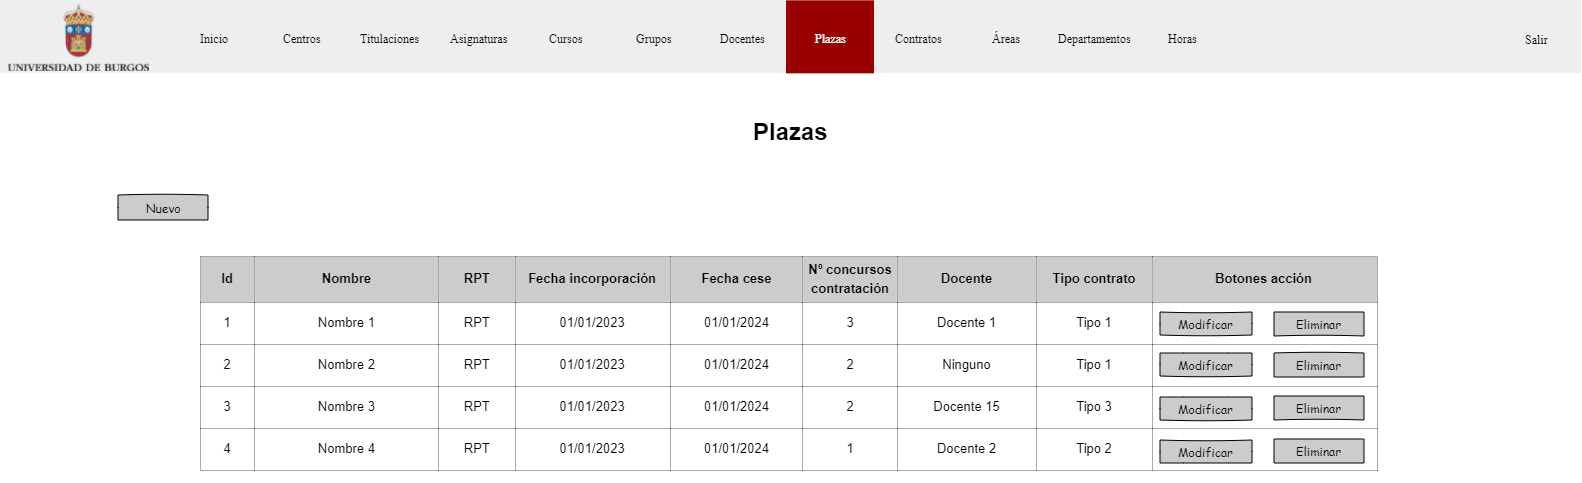
\includegraphics[width=\textwidth]{../img/Anexos/Vistas/plazas.png}
		\caption{Mantenimiento de plazas}\label{F-CU2.5}
		\end{figure}
		\FloatBarrier
\newpage
		\item \textbf{CU-2.5.1} Añadir/Modificar plazas. Ver figura~\ref{F-CU2.5.1}
		\begin{figure}[!h]
		\centering
		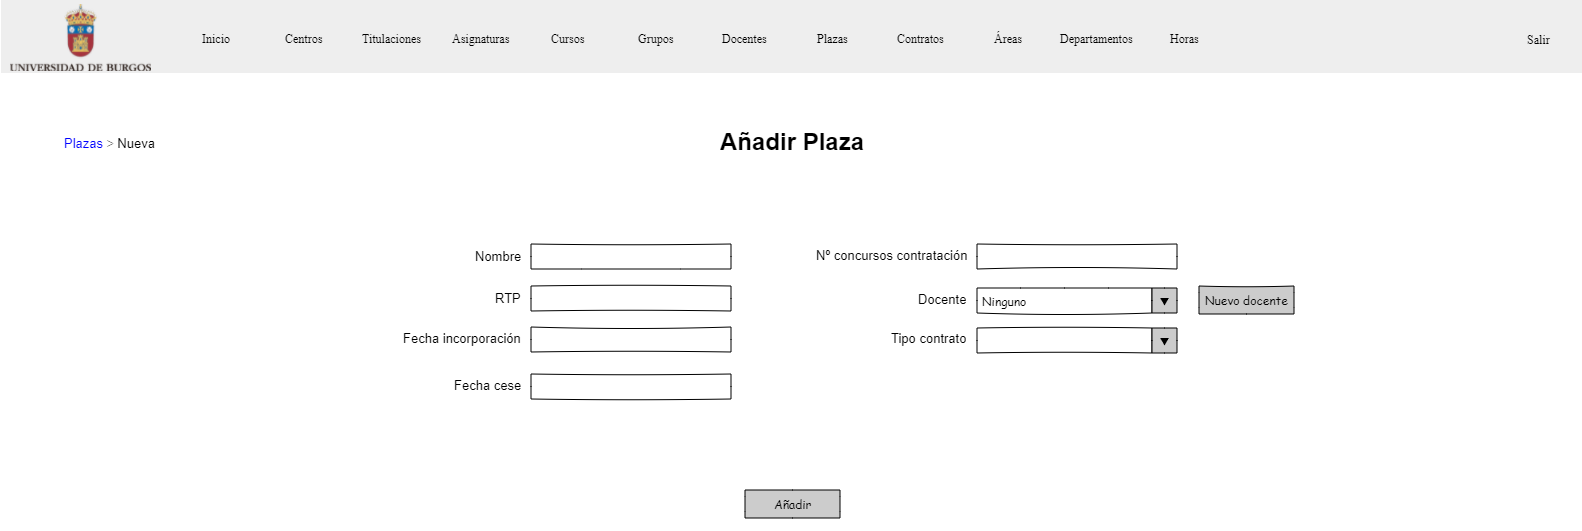
\includegraphics[width=\textwidth]{../img/Anexos/Vistas/add_plaza.png}
		\caption{Añadir/Modificar plazas}\label{F-CU2.5.1}
		\end{figure}
		\FloatBarrier
		\item \textbf{CU-2.6} Asignar plaza a docente. Ver figura~\ref{F-CU2.6}
		\begin{figure}[!h]
		\centering
		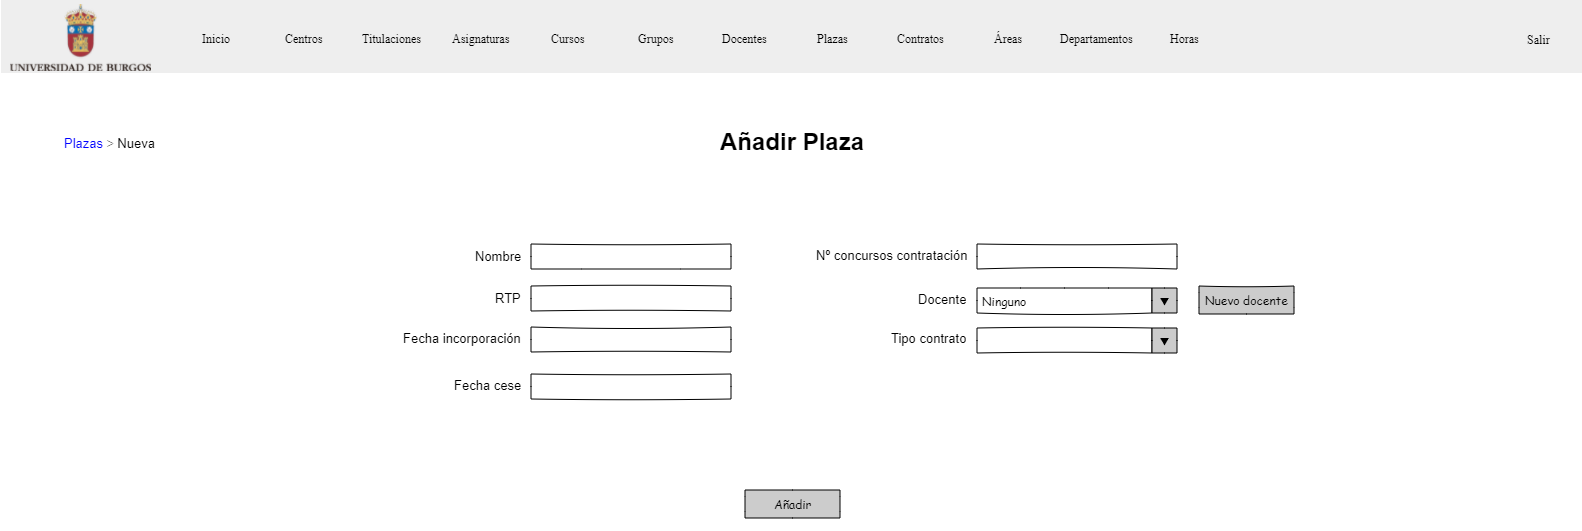
\includegraphics[width=\textwidth]{../img/Anexos/Vistas/add_plaza.png}
		\caption{Asignar plaza a docente}\label{F-CU2.6}
		\end{figure}
		\FloatBarrier
	\end{itemize}
	
\newpage
	\item \textbf{CU-3.} Asignación docente.
	\begin{itemize}
		\item \textbf{CU-3.1} Mantenimiento cursos académicos. Ver figuras~\ref{F-CU3.1} y~\ref{F-CU3.1(1)}
		\begin{figure}[!h]
		\centering
		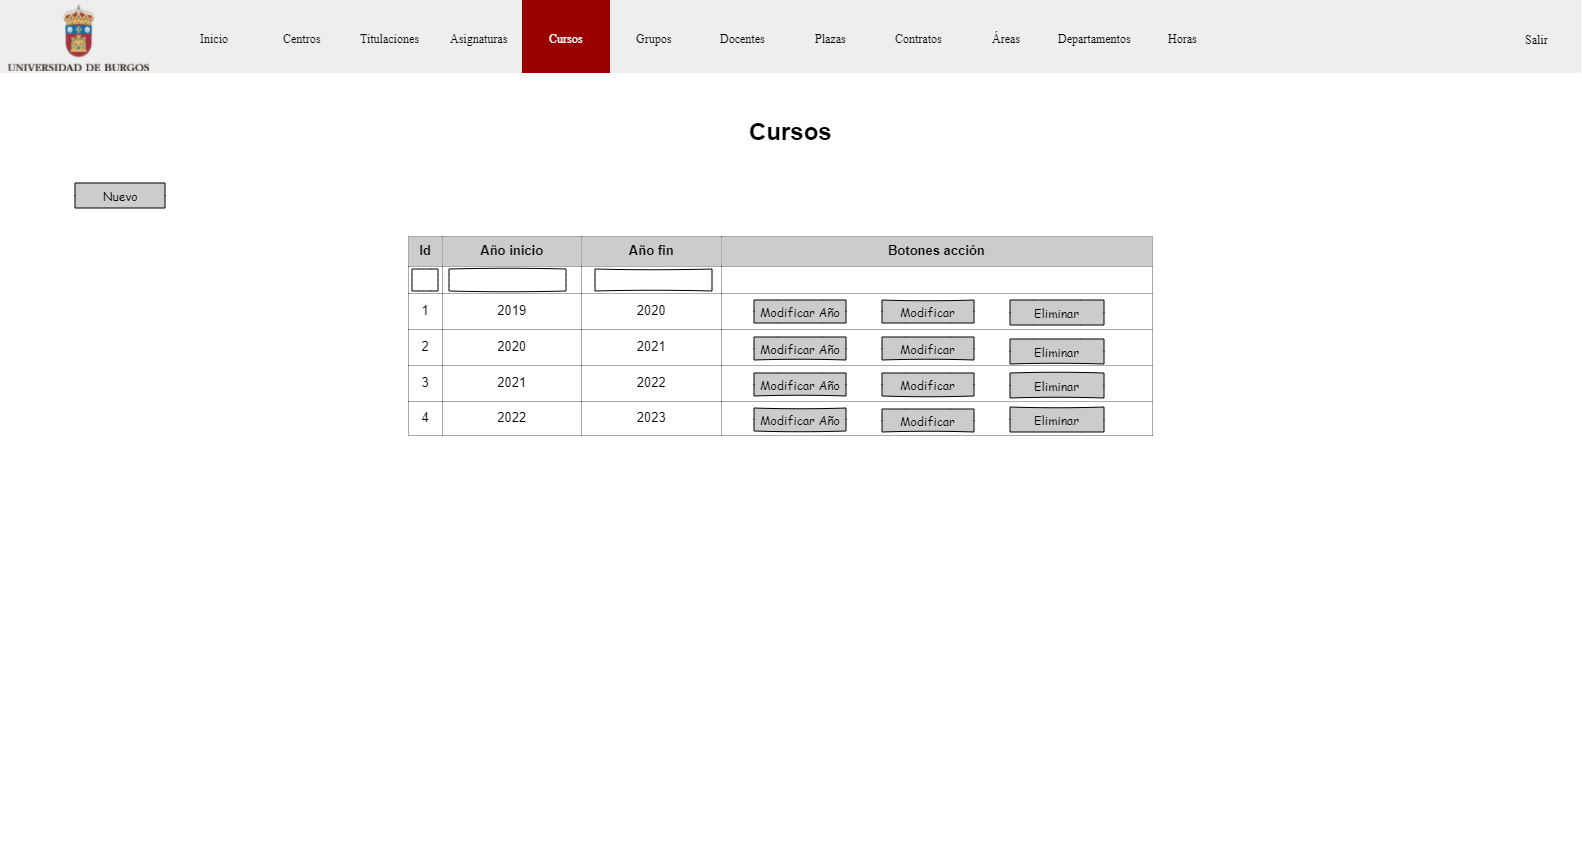
\includegraphics[width=\textwidth]{../img/Anexos/Vistas/cursos.png}
		\caption{Mantenimiento cursos académicos}\label{F-CU3.1}
		\end{figure}
		\FloatBarrier
		\begin{figure}[!h]
		\centering
		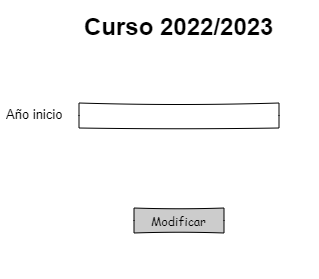
\includegraphics[width=0.5\textwidth]{../img/Anexos/Vistas/mod_ano_curso.png}
		\caption{Modificar año curso académico}\label{F-CU3.1(1)}
		\end{figure}
		\FloatBarrier
\newpage
		\item \textbf{CU-3.1.1} Añadir curso académico. Ver figuras~\ref{F-CU3.1.1} y~\ref{F-CU3.1.1(1)}
		\begin{figure}[!h]
		\centering
		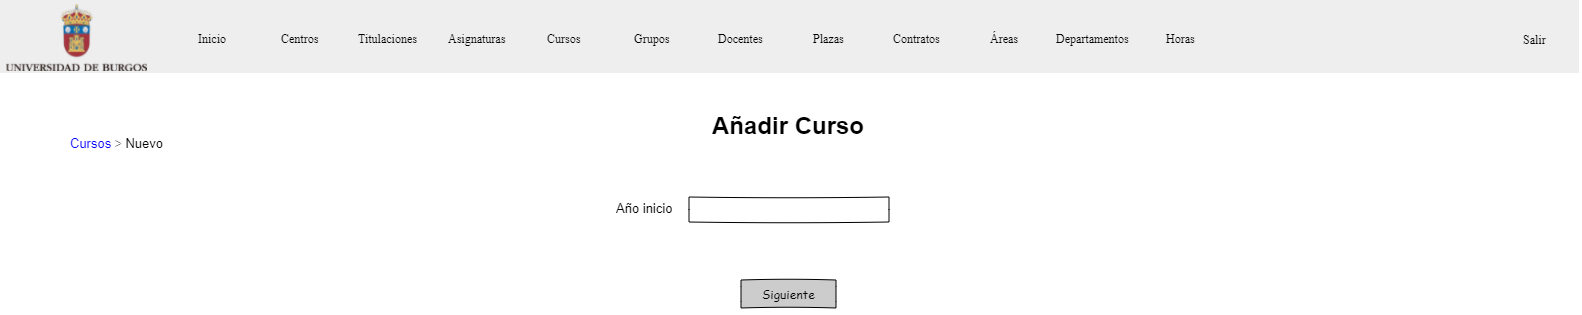
\includegraphics[width=\textwidth]{../img/Anexos/Vistas/add_curso.png}
		\caption{Añadir curso académico}\label{F-CU3.1.1}
		\end{figure}
		\FloatBarrier
		\begin{figure}[!h]
		\centering
		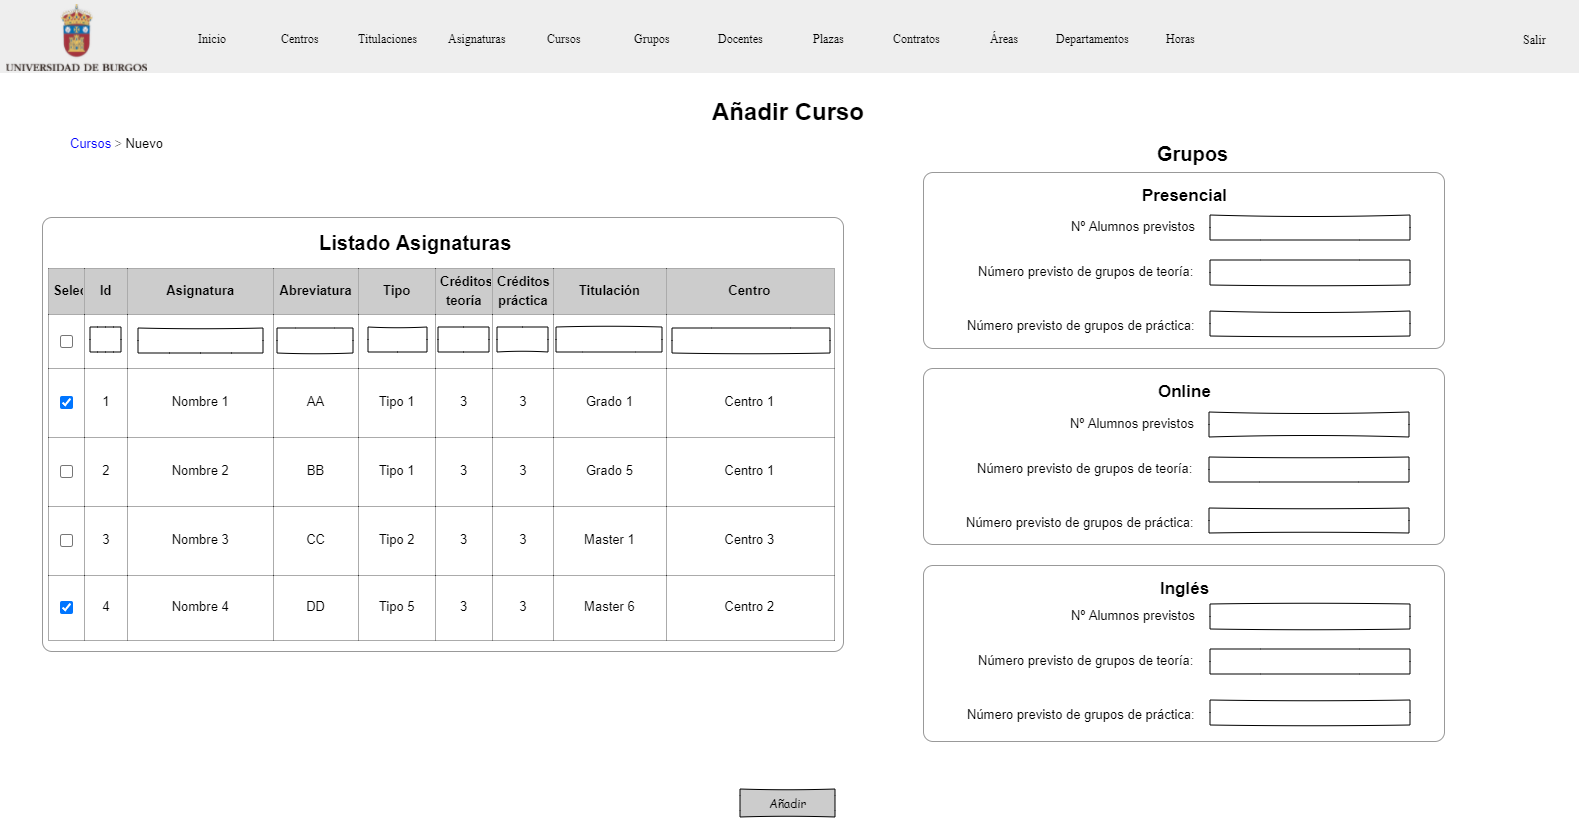
\includegraphics[width=\textwidth]{../img/Anexos/Vistas/add_curso_1.png}
		\caption{Añadir curso académico 2}\label{F-CU3.1.1(1)}
		\end{figure}
		\FloatBarrier
\newpage
		\item \textbf{CU-3.1.2} Modificar curso académico. Ver figuras~\ref{F-CU3.1.2} y~\ref{F-CU3.1.2(1)}
		\begin{figure}[!h]
		\centering
		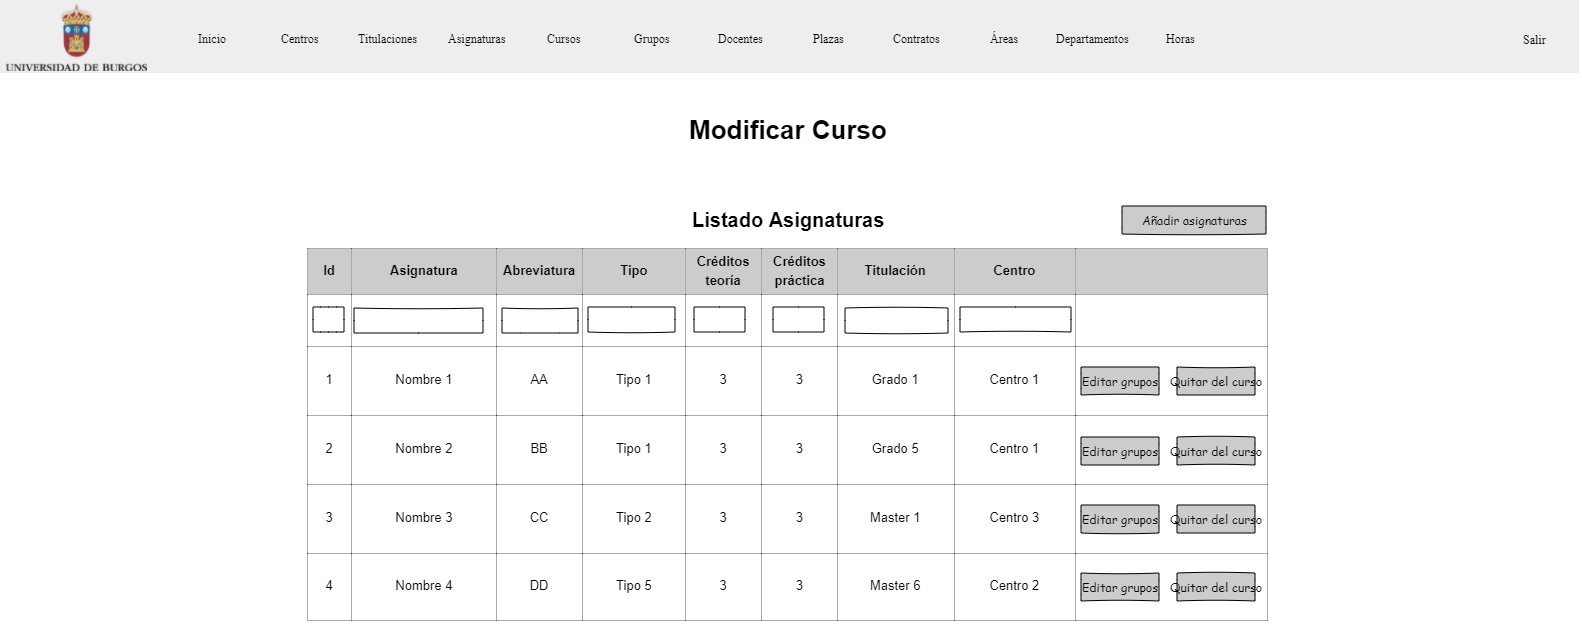
\includegraphics[width=\textwidth]{../img/Anexos/Vistas/mod_curso.png}
		\caption{Modificar curso académico}\label{F-CU3.1.2}
		\end{figure}
		\FloatBarrier
		\begin{figure}[!h]
		\centering
		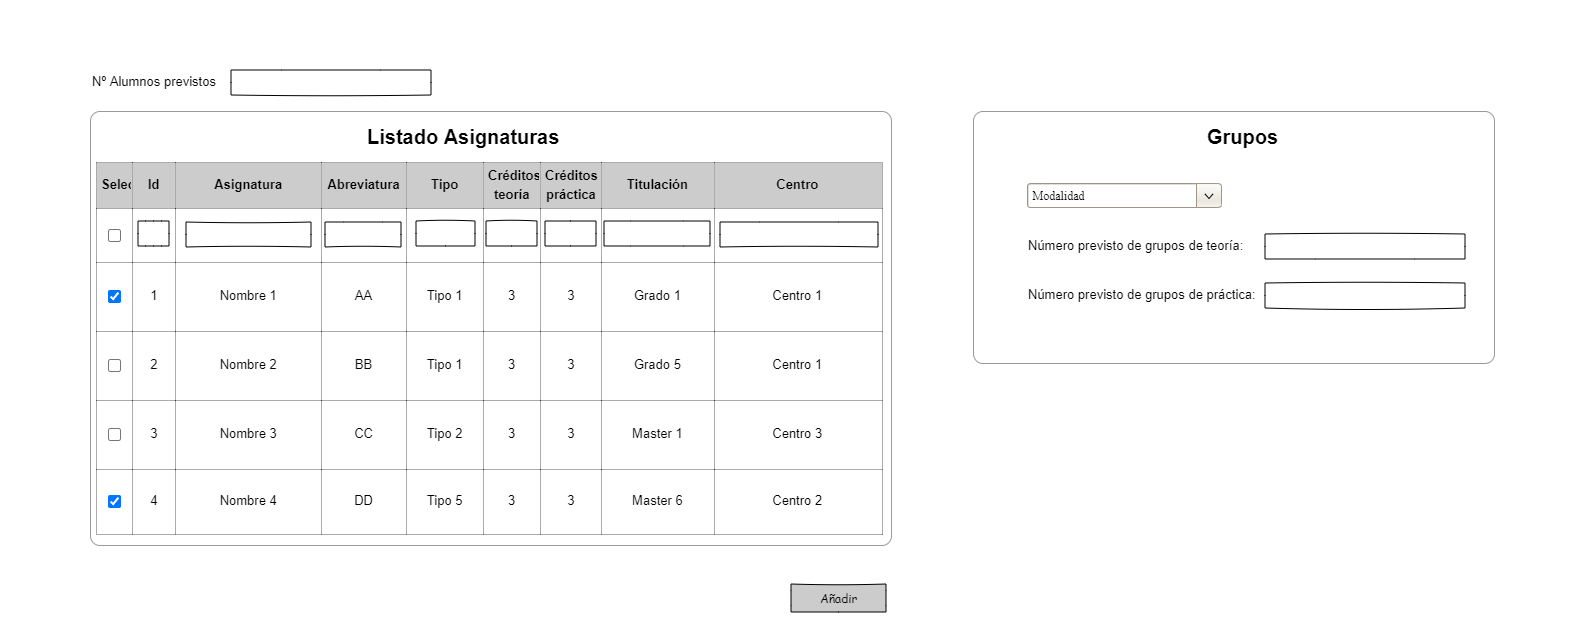
\includegraphics[width=\textwidth]{../img/Anexos/Vistas/add_asig.png}
		\caption{Añadir asignaturas al curso}\label{F-CU3.1.2(1)}
		\end{figure}
		\FloatBarrier
\newpage
		\item \textbf{CU-3.2} Mantenimiento de grupos. Ver figura~\ref{F-CU3.2} 
		\begin{figure}[!h]
		\centering
		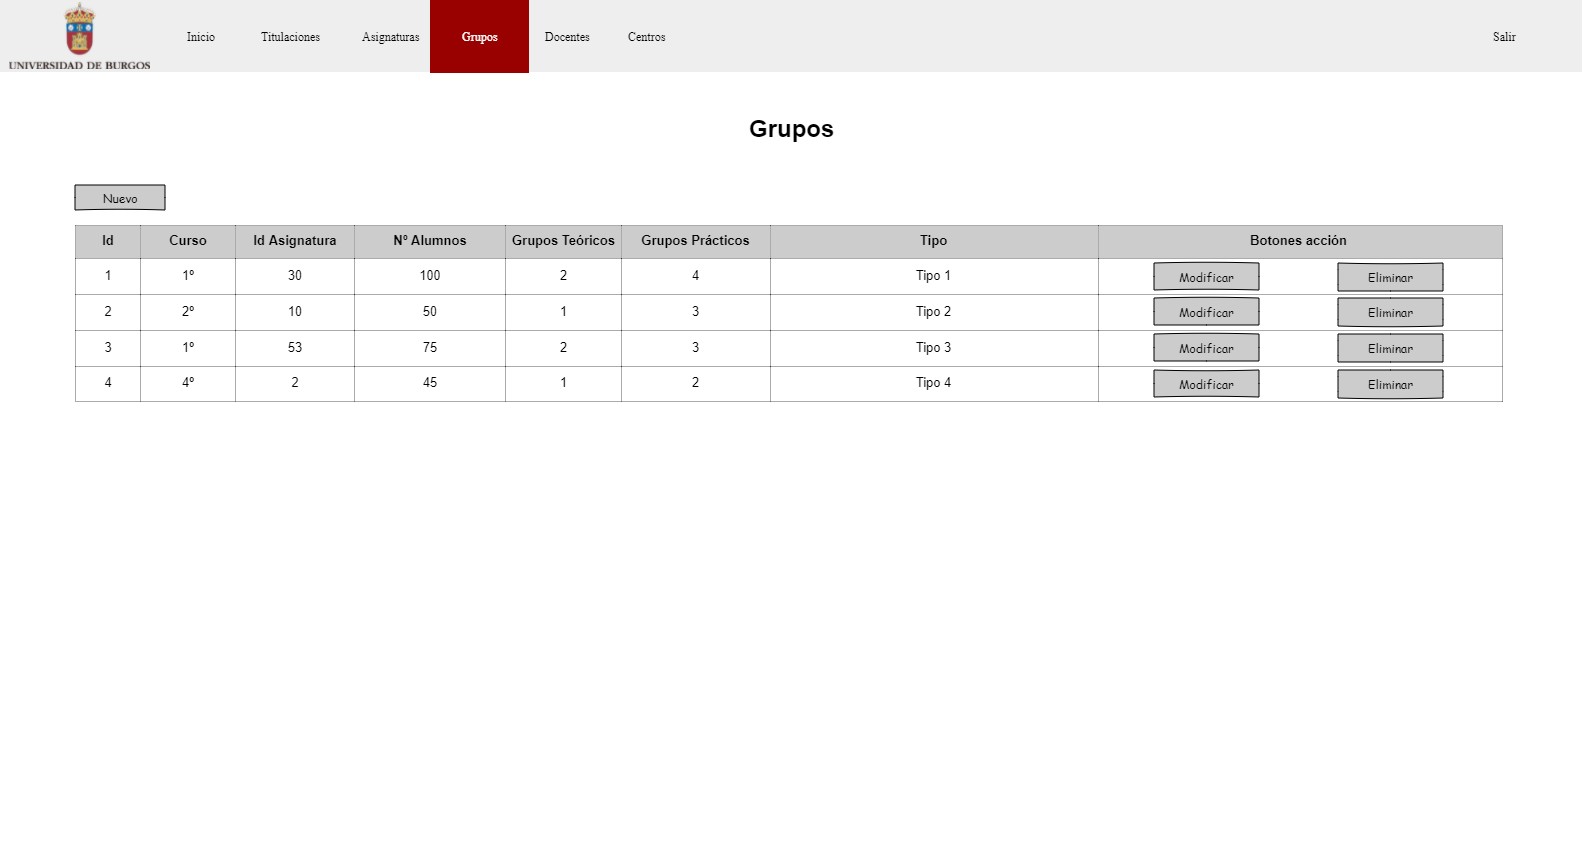
\includegraphics[width=\textwidth]{../img/Anexos/Vistas/grupos.png}
		\caption{Mantenimiento de grupos}\label{F-CU3.2}
		\end{figure}
		\FloatBarrier
		\item \textbf{CU-3.2.1} Añadir/Modificar grupo. Ver figuras~\ref{F-CU3.2.1} y~\ref{F-CU3.2.1(1)}  
		\begin{figure}[!h]
		\centering
		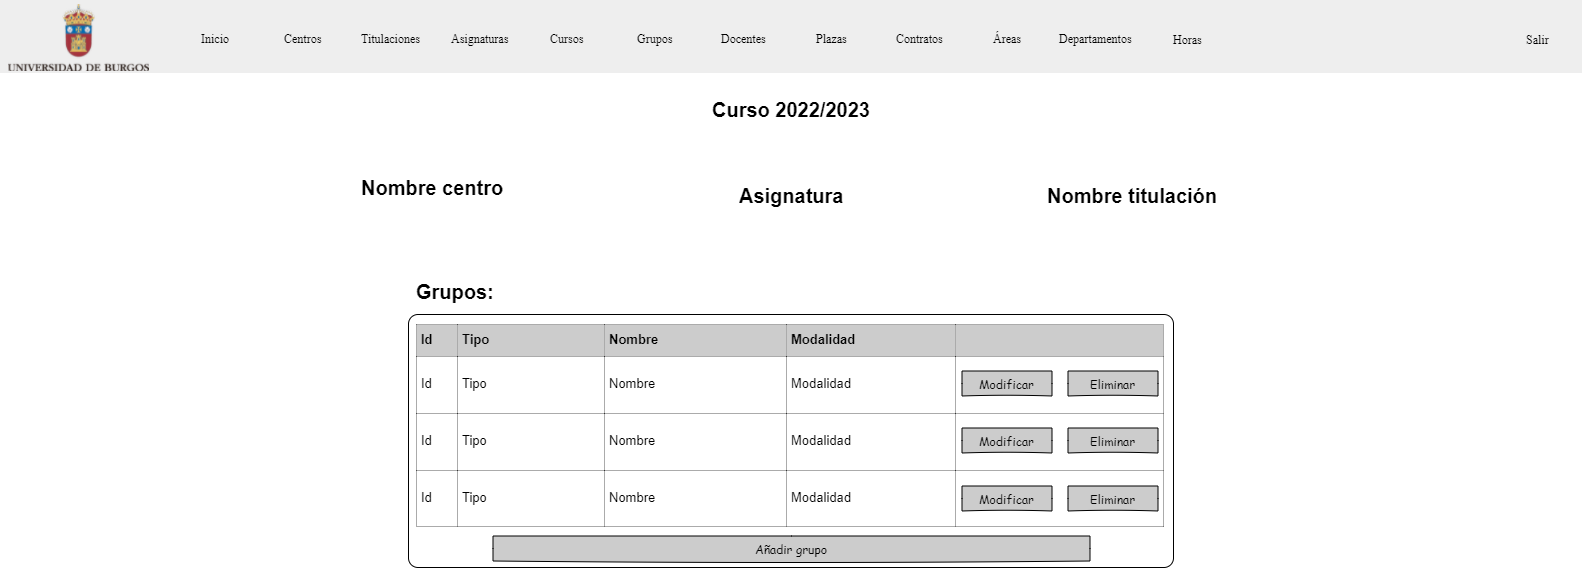
\includegraphics[width=\textwidth]{../img/Anexos/Vistas/addmod_grupo.png}
		\caption{Añadir/Modificar grupo}\label{F-CU3.2.1}
		\end{figure}
		\FloatBarrier
		\begin{figure}[!h]
		\centering
		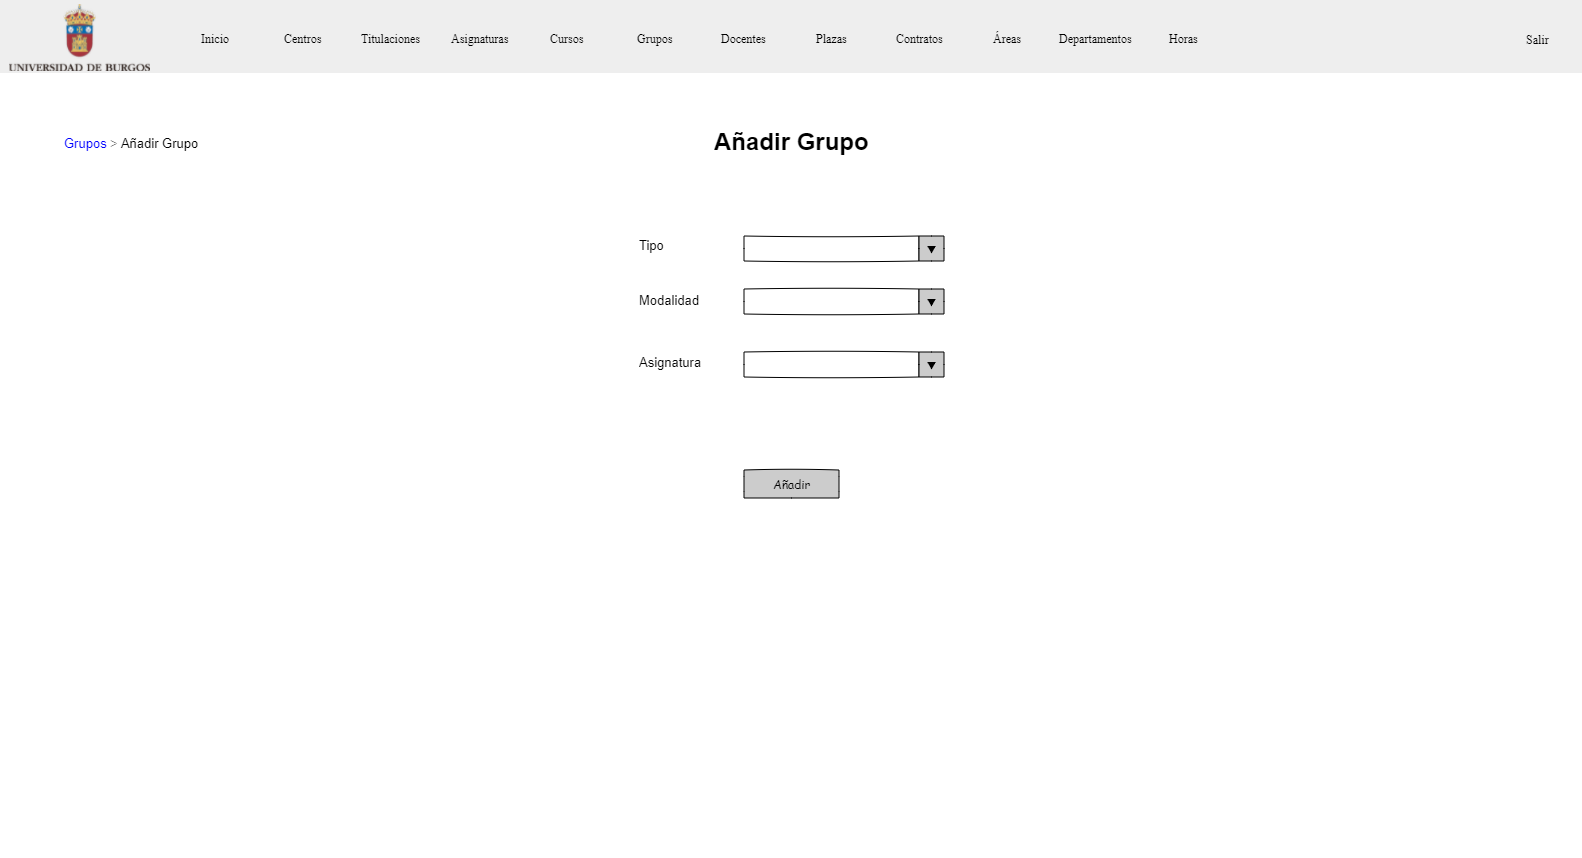
\includegraphics[width=0.5\textwidth]{../img/Anexos/Vistas/add_grupo.png}
		\caption{Añadir/Modificar grupo 2}\label{F-CU3.2.1(1)}
		\end{figure}
		\FloatBarrier
		\newpage
		\item \textbf{CU-3.3} Asignación de horas de plazas a grupos. Ver figuras~\ref{F-CU3.3},~\ref{F-CU3.3(1)} y~\ref{F-CU3.3(2)} 
		\begin{figure}[!h]
		\centering
		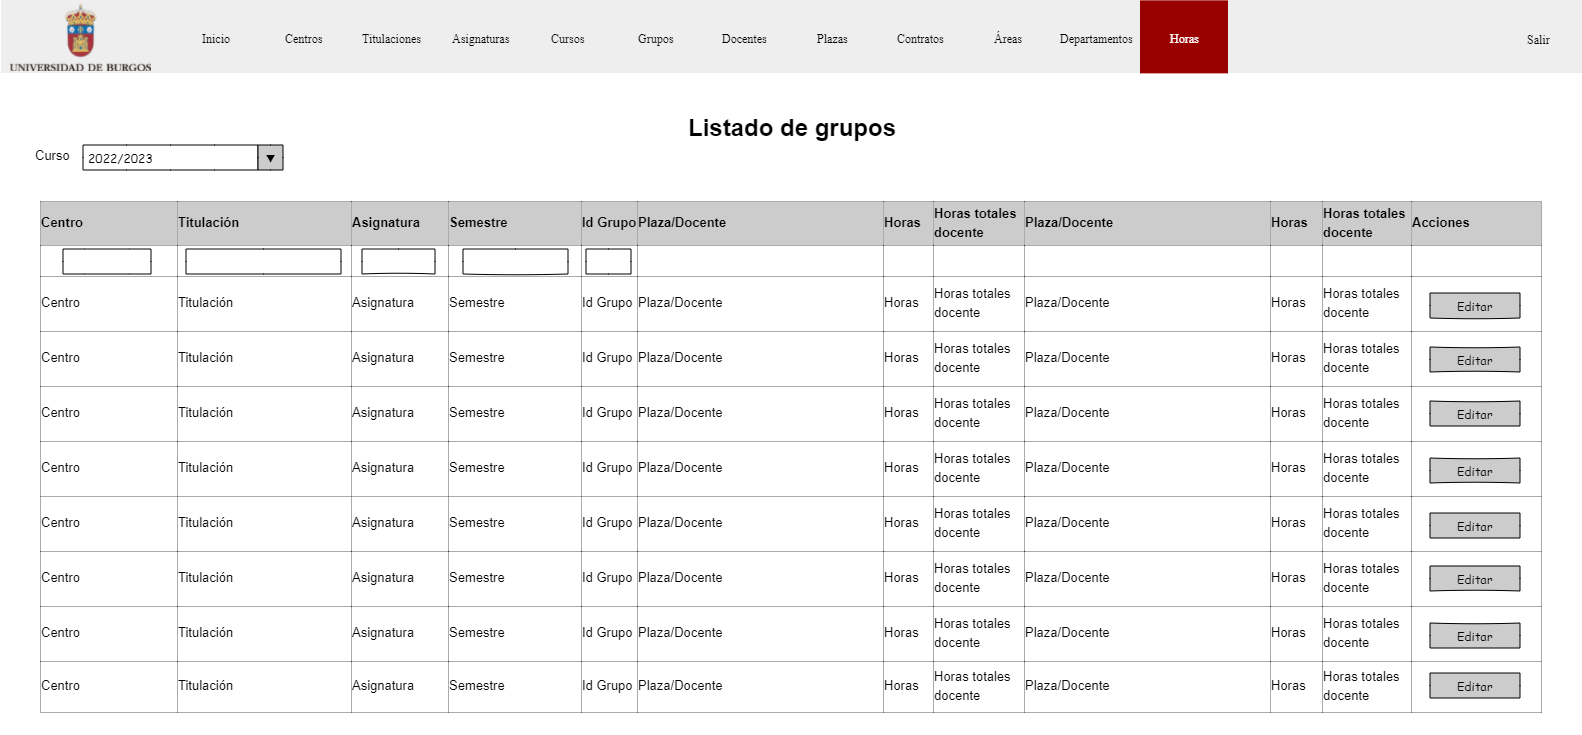
\includegraphics[width=\textwidth]{../img/Anexos/Vistas/horas.png}
		\caption{Asignación de horas de plazas a grupos}\label{F-CU3.3}
		\end{figure}
		\FloatBarrier
		\begin{figure}[!h]
		\centering
		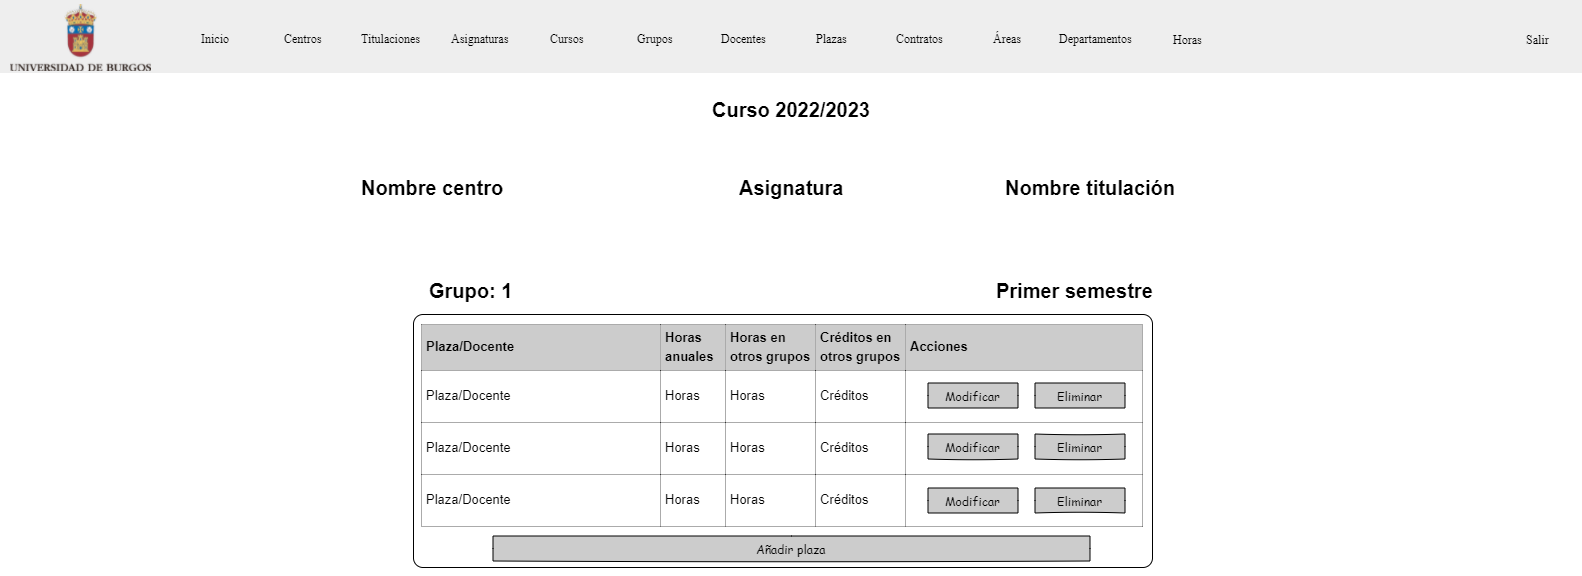
\includegraphics[width=\textwidth]{../img/Anexos/Vistas/asig_horas_plaza_grupo.png}
		\caption{Asignación de horas de plazas a grupos 2}\label{F-CU3.3(1)}
		\end{figure}
		\FloatBarrier
		\begin{figure}[!h]
		\centering
		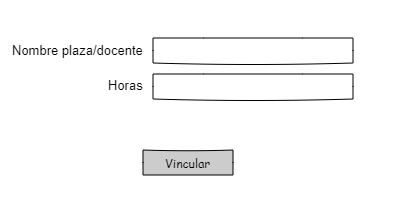
\includegraphics[width=0.5\textwidth]{../img/Anexos/Vistas/asig_horas_plaza_grupo_modal.png}
		\caption{Asignación de horas de plazas a grupos 3}\label{F-CU3.3(2)}
		\end{figure}
		\FloatBarrier
	\end{itemize}
\end{itemize}


